\chapter{Theoretical Model}
In this chapter, the mathematical basis for \textit{omnisoot} is explained in the top-to-bottom hierarchical order. The highest level is the reactors and flames that include the transport equations of gas mixture and "soot variables". Soot formation source terms are handled by the particle dynamics model that mainly addresses particle size distribution (PSD), morphology and coagulation rate. The "PAH growth model" computes the contribution of inception and adsorption to source terms based on PAHs designated as precursors. Similarly, the "surface reactions" model obtains the surface growth and oxidation rate by HACA mechanism and passes them to the particle dynamics model. 

\section{Assumptions and conventions}
Here, the main conventions and assumptions used in the derivation of the mathematical model are listed below.

\begin{enumerate}
\item The ideal gas law is used to calculated physical, transport, and chemical properties of gas mixture.
	
\item $\mathrm{\dot{s}_k}$ denotes that rate production/consumption of $k_{th}$ species due to soot formation. It is positive when the species is released to gas mixture.

\item Each soot agglomerate consist of spherical monodisperse primary particles in point contact.

\item The word \textit{``particle"} refers to soot both in spherical and agglomerate shape. 

\item The density of soot is assumed constant at the value of 1800 $\mathrm{kg/m^3}$. This density represents an average between particles with small C/H ratio ($\mathrm{\rho=1600 kg/m^3}$) and large C/H ratios ($\mathrm{\rho=2000 kg/m^3}$)~\citep{jensen2007measurement}.

\item The incipient soot particles are 2~nm in diameter, so no particles could exist with a primary particle diameter smaller than 2~nm. The number of carbon atoms in the incipient soot particle is calculated from the mass of a sphere with the diameter of 2~nm assuming pure carbon content.
\begin{equation}
	\begin{split}
	d_{p,min}&=2~\mathrm{nm} \\
	n_{c,min}& =\frac{\pi}{6}\rho_{soot}d^3_{p,min}\frac{1}{MW_c}\approx378
	\label{eqn:dp_min}.
	\end{split}
\end{equation}
\item The calculation of PAH adsorption and soot oxidation requires ``\textit{soot concentration}" which is defined as the number of soot agglomerates per unit volume of gas. The number density of agglomerates,  $\mathrm{N_{agg}}$, are tracked per unit mass of gas mixture i.e. $\mathrm{\#/kg_{gas}}$. So, soot concentration can be calculated by multiplying agglomerate number density by gas density as:
\begin{equation}
	[\mathrm{soot}] = \rho\cdot \mathrm{N_{agg}}
	\label{eqn:sootconcen}.
\end{equation}

\item The specific heat, internal energy and enthalpy of soot are approximated by those of pure graphite, and employed to close the energy balance in the system~\cite{mcbride1993coefficients}.

\item Soot particles and gas are in thermal equilibrium during studied processes.

\item There is no temperature gradient within each agglomerate.

\item \textit{Soot variable} refers to the features/properties of soot particles tracked by the particle dynamics model and used in the soot transport equations.

\item \textit{PAH growth} is a unit of the soot model with a set of pathways that determine the rate of inception and adsorption from PAHs in the gas mixture.

\item \textit{Surface reactions} is a unit of the soot model that describes the addition of acetylene to soot surface, and removal of carbon via oxidation by OH and $\mathrm{O_2}$ in the HACA scheme.

\item The superscript \textit{i} denotes section number of a soot variable or property derived from variables. In the case of the monodisperse model, the section number can be ignored because it is equivalent to the sectional model with one section.

\item The computation of morphological parameters ($d_p$, $d_m$, $d_g$, and $n_p$) and diffusion coefficient are done similarly by both particle dynamics models, so they are explained separately in standalone sections.

\end{enumerate}

\section{Flames}
This research focuses on axisymmetric stagnation flames that reduces the laminar 3D steady-state equations in the cylindrical coordinates (r-z-$\mathrm{\theta}$ system) to one-dimensional domain in r-z plane. The derivation of flow equations for a reacting gas is explained in detail in Section 7.2 of \citep{kee2017chemically}. Here, the modified version of equations is provided that takes into account the mass and momentum of particles, the removal/release of species due to soot inception, surface growth and oxidation as well as the formation and sensible energy of soot.

\noindent Continuity:
\begin{equation}
	\frac{\partial \rho u}{\partial z} = 2\rho V - \sum_j \dot{s}_j W_j
	\label{eqn:flame_cont},
\end{equation}

\noindent Radial Momentum:
\begin{equation}
	\rho u\frac{\partial V}{\partial z} + \rho V^2=-\Lambda +
	\frac{\partial}{\partial z}
	\left(
		\mu \frac{\partial V}{\partial z}
	\right)
	\label{eqn:flame_momen},
\end{equation}
\noindent Energy:
\begin{equation}
	\left[
		(1-\varphi)\rho c_p
		+\varphi\rho_{soot} c_{p,soot}
	\right] u
	\frac{\partial T}{\partial z} = 	\frac{\partial}{\partial z}
	\left(
	K \frac{\partial T}{\partial z}
	\right)
	-\sum_{k}^{n_{sp}} J_k \frac{\partial h_k}{\partial z}
	-\sum_{k}^{n_{sp}} h_k W_k
	\left(
		\omega_k+\dot{s}_k
	\right)
	\label{eqn:flame_energy},
\end{equation}
\noindent Species:
\begin{equation}
	\rho u\frac{\partial Y_k}{\partial z} = 
	-\frac{\partial J_k}{\partial z}
	+ W_j 
	\left(
	\omega_k+\dot{s}_k
	\right)
	\label{eqn:flame_species},
\end{equation}
\noindent where $\mathrm{V=v/r}$ is the scaled radial velocity, and $\mathrm{\Lambda}$ is the pressure eigenvalue. $\mathrm{J_k}$ denotes the diffusive flux of species $\mathrm{k}$ that is usually calculated using mixture averaged formulation.

\begin{equation}
	J^*_K = -\rho \frac{W_k}{W_T}D^{'}_{km}
	\frac{\partial X_k}{\partial z}
	\label{eqn:diffflux_star},
\end{equation}

\begin{equation}
	J_K = J^*_K - Y_k \sum_{l=1}^{n_{sp}} J^*_l
	\label{eqn:diffflux},
\end{equation}

The details of calculation of mixture-averaged diffusive fluxes can be found in the documentation of \verb| GasTransport::getMixDiffCoeffs()|\footnote[1]{https://cantera.org/documentation/docs-3.0/doxygen/html/d8/d58/classCantera\_1\_1GasTransport.html} in Cantera~\citep{cantera}. Soot variables are treated similar to species, and their transport equations can be written as:
\begin{equation}
	\rho u\frac{\partial \psi}{\partial z} = 
	-\frac{\partial}{\partial z}
	\left(
		D\frac{\partial \psi}{\partial z}
	\right)
	+ S_{\psi} 
	\label{eqn:flame_soot},
\end{equation}
\noindent where $\psi$ is a generic soot variable that represents any of tracked soot variables.

\section{Reactors}
Zero-dimensional reactors are ideal representation of reactive systems typical in industrial applications. The strong mixing in the volume/cross-section allows description of thermal/chemical/hydrodynamic properties of mixture with a single variable that evolves in time. This section entails the conservation equations of mass, momentum (if applicable), species, energy, and soot for three reactor models.

\subsection{Constant Volume Reactor}
This reactor assumes that the volume of system does not change during the process. In the absence of soot, this leads to gas with constant density. However, soot formation converts part of gaseous species to solid particles thereby affecting its volume and density. Note that, continuity, species and energy transport equations only track gas mixture properties. Figure~\ref{fig:constuvcv} illustrates the control volume over the gas mixture targeted by mass and energy balance equations. Any mass converted to solid soot particles leaves the control volume. Mass and energy passes through the control surface around solid particles by soot formation processes. Reactor volume is the sum of volume of gas mixture and solid particles.

\begin{figure}[!htbp]
	\centering
	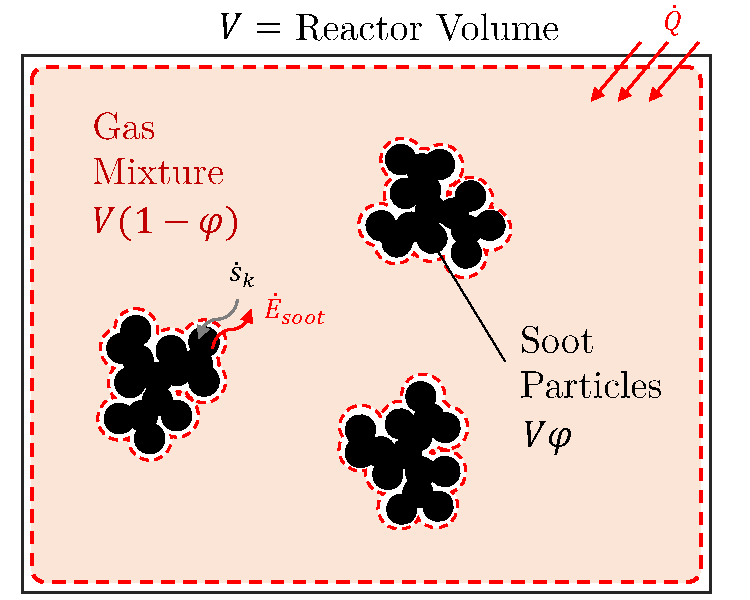
\includegraphics[height=50mm, ]{Figures/Theory/ConstUV.pdf}
	\caption{The schematics of control volume considered for the constant volume reactor that encompasses the gas mixture and excludes the soot particles. Mass and energy are transferred between gas and soot particles.}
	\label{fig:constuvcv}
\end{figure}
 
The continuity for this reactor can be written as:

\begin{equation}
	\frac{d}{dt}(\rho(1-\varphi)) =(1-\varphi) \sum_i \dot s_i W_i
	\label{eqn:contconstuv}.
\end{equation} 

Similarly, the species equation for species $k$ is expressed as:

\begin{equation}
	\frac{dY_k}{dt}
	=
	\frac{1}{\rho}
	\left(
		{\dot{\omega}}_k
		+
		{\dot{s}}_k
	\right)W_k
	-\frac{1}{\rho}Y_k\sum_{i}{{\dot{s}}_i W_i}
	\label{eqn:speciesconstuv}.
\end{equation}

The energy balance for the gas mixture can be simplified to the rate of change of temperature. An external heat source of $\mathrm{\dot{Q}}$ is considered to account for possible heat loss/gain of the reactor.
\begin{equation}
	\frac{d T}{d t}=
	\frac{1}{\rho (1-\varphi) c_v+\rho_{soot}\varphi c_{v,soot}}
	\left[
		-(1-\varphi)\sum_k e_k
			\left(
				\dot{\omega}_k+\dot{s}_k
			\right) W_k
		+u_{soot}(1-\varphi)\sum_k \dot{s}_k W_k
		+\frac{\dot{Q}}{V}
	\right]
	\label{eqn:energyconstuv}.
\end{equation}



The transport equation for a generic soot variable, $\psi$ can be written as:
\begin{equation}
	\frac{d \psi}{d t}= S_{\psi} - \frac{\psi}{\rho} \sum_i \dot{s}_i W_i
	\label{eqn:sootconstuv}.
\end{equation}

\subsection{Perfectly Stirred Reactor}
In this reactor, gas enters with a mass flow rate $\dot{m_{in}}$, composition of $Y^\ast$ and temperature of $T^\ast$, instantaneously mixes and homogeneously reacts with the mixture resident inside the reactor. The reacting gas reaches a spatially uniform temperature and composition described by $T$, and $Y$. It is assumed that temperature, composition and soot properties of the outflow are the same as reactor. Figure~\ref{fig:psrcv} illustrates the schematics of PSR. $\mathrm{\dot{m}_{in}}$ and $\mathrm{\dot{m}_{out}}$ refer to inflow and outflow gas mass flow rates, respectively. Under no-soot conditions, the inlet and outlet mass flow rates are equal, but the gas mixture loses mass by soot formation, so $\mathrm{\dot{m}_{out}}$ is slightly less than $\mathrm{\dot{m}_{in}}$. The pressure of reactor is assumed to stay constant during the process~\citep{kee2017chemically}. The nominal residence time of gas mixture in the reactor is defined as:

\begin{equation}
	\tau = \frac{\rho V}{\dot{m}_{in}}
	\label{eqn:taupsr}.
\end{equation} 

 

\begin{figure}[!htbp]
	\centering
	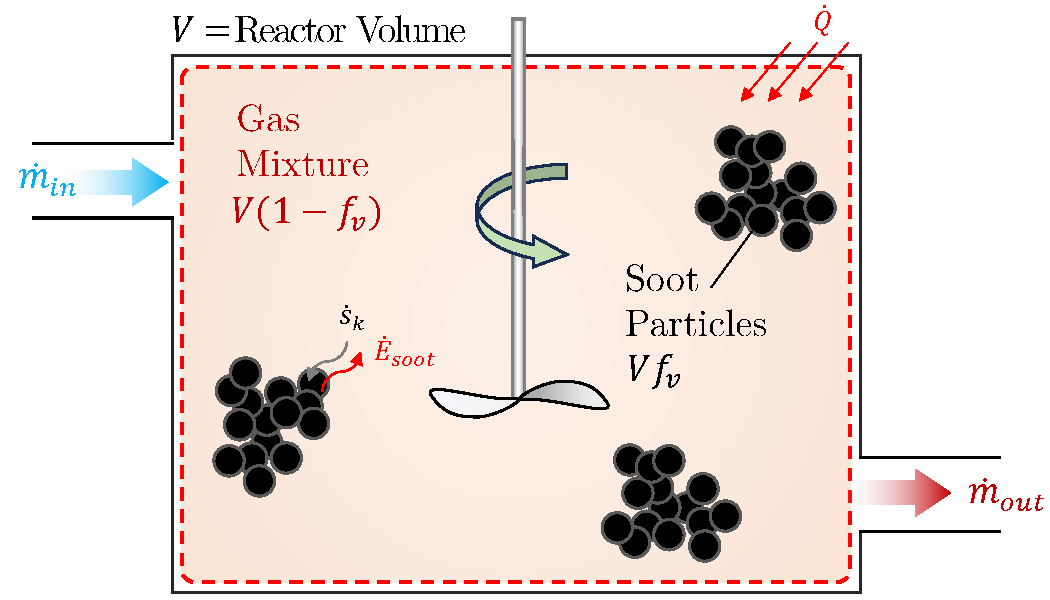
\includegraphics[height=50mm, ]{Figures/Theory/PSR.pdf}
	\caption{The schematics of control volume considered for the perfectly stirred reactor that encompasses the gas mixture and excludes the soot particles. Mass and energy are transferred between gas and soot particles. The inlet flow brings species and enthalpy into the control volume and the outlow discharges them. The outflow  mass flow is less than inflow mass flow due to soot formation.}
	\label{fig:psrcv}
\end{figure}

The conservation of mass can be written for PSR by considering the mass flux of in- and outflow, and the removal of mass due to soot generation as:

\begin{equation}
	\frac{d m}{d t}
	=
	\dot{m}_{in} - \dot{m}_{out} 
	+ (1-\varphi) \sum_i \dot{s}_i W_i 
	\label{eqn:contpsr}.
\end{equation}

The density is not determined by solving the continuity equation, but rather from ideal gas law and assuming a constant pressure and the composition from solving the species transport equations as:

\begin{equation}
	\frac{d Y_k}{d t}
	=
	\frac{1}{\tau}
	\left( Y^*_k-Y_k \right)+
	\frac{1}{\rho}\left[\left(\dot{\omega}_k+\dot{s}_k\right) W_k-Y_k \sum_i \dot{s}_i W_i\right]
	\label{eqn:speciespsr}.
\end{equation}

The energy equation for this reactor is written as:
\begin{equation}
	\begin{split}
		\frac{dT}{dt}
		=
		\frac{1}
		{
			\rho\left(1-\varphi\right)c_p+\rho_{soot}c_{p,soot}\varphi
		}
		\left[
		\frac{{\dot{m}}_{in}}{V}
		\left(h^\ast-h\right)
		-
		\frac{{\dot{m}}_{in}}{V}\sum_{k}\left(Y_k^\ast-Y_k\right)h_k
		\right.\\
		\left.	
		-
		\left(1-\varphi\right)\sum_{k}{
			\left(
			{\dot{\omega}}_k
			+
			{\dot{s}}_k
			\right) W_k h_k}
		+\left(1-\varphi\right) \sum_{i}{{\dot{s}}_i W_i} h_{soot}+\frac{\dot{Q}}{V}
		\right].
	\end{split}
		\label{eqn:energypsr}
\end{equation}

The soot transport equations can also be expressed as:
\begin{equation}
	\frac{d\psi}{dt}
	=
	\frac{{\dot{m}}_{in}}{\rho V
	\left(1-\varphi\right)}
	\left(\psi^\ast-\psi\right)
	+
	S_{\psi}
	-\frac{1}{\rho}\psi\sum_{i}{{\dot{s}}_i W_i}
	\label{eqn:sootpsr}.
\end{equation}

\subsection{Plug Flow Reactor}
The plug flow reactor (PFR) is an ideal representation of a channel or duct with a constant cross-sectional area where a steady-state one-dimensional flow changes temperature, composition, and soot properties along the channel. There is no spatial gradient over the cross-section due to strong mixing. Diffusion along the channel is negligible. The pressure is assumed constant along the reactor.
\begin{figure}[!htbp]
	\centering
	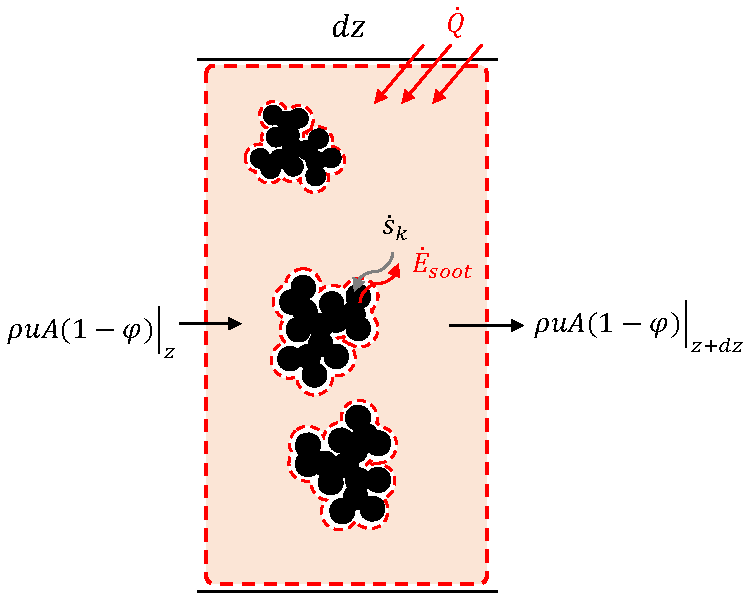
\includegraphics[height=50mm, ]{Figures/Theory/PFR.pdf}
	\caption{The schematics of control volume for a differential element along PFR that includes the gas mixture and excludes the soot particles considering wall heat transfer. Mass and energy are transferred between gas and soot.}
	\label{fig:pfrcv}
\end{figure}


The continuity equation for PFR is written as:
\begin{equation}
	\frac{d}{dz}(\rho u(1-\varphi)) =(1-\varphi) \sum_i \dot s_i W_i
	\label{eqn:contpfr}.
\end{equation}

The momentum equation can also be established as:
\begin{equation}
	u (1-\varphi) \sum_i \dot s_i W_i + \rho u (1-\varphi) \frac{du}{dz}
	=-\frac{d}{dz}(P(1-\varphi))-\frac{\tau_{w}}{\mathrm{R_H}} 
	\label{eqn:momenpfr}.
\end{equation}
\noindent where $\tau_w$ is the wall shear the can be determined from fraction factor, $f$ as:
\begin{equation}
	\tau_w = \frac{1}{2}\rho u^2 f 
	\label{eqn:wallshearpfr}.
\end{equation}

The friction factor, $f$ can be calculated with a good accuracy for the entire range of Reynolds number, Re, from laminar to turbulent flow using the explicit formula given by \citet{haaland1983simple}:

\begin{equation}
	\frac{1}{f^{1/2}} = -1.8 \mathrm{log}
	\left(
		\frac{6.9}{Re}+
		\left[ \frac{\epsilon/D_H}{3.7} \right]^{1.11}
	\right)
	\label{eqn:fpfr},
\end{equation}
\noindent where $\epsilon$ is the roughness of reactor wall.
$\mathrm{R_H}$ and $\mathrm{D_H}$ are hydraulic radius and diameter, respectively that can be determined from cross-section geometry of reactor as:

\begin{equation}
	D_H = 4 R_H = \frac{4 A_c}{P_c}
	\label{eqn:RDHpfr},
\end{equation}
\noindent $A_c$ and $P_c$ are cross-sectional area and wetted perimeter of the reactor.
The species equation can be expressed as:
\begin{equation}
	\frac{d Y_k}{d z}=\frac{1}{\rho u}\left[\left(\dot{\omega}_k+\dot{s}_k\right) W_k-Y_k \sum_i \dot{s}_i W_i\right]
	\label{eqn:speciespfr}.
\end{equation}

The energy equation can be expressed as:
\begin{equation}
	\begin{split}
		\frac{d T}{d z}=
		\frac{1}{\rho u (1-\varphi) c_p+\rho_{soot} u \varphi 	c_{p,soot}}
		\left[
			-(1-\varphi)\sum_k h_k
			\left(
			\dot{\omega}_k+\dot{s}_k
			\right) W_k
		\right. \\
		\left.
			+h_{soot}(1-\varphi)\sum_k \dot{s}_k W_k
			+\dot{q}^\prime
		\right]
	\end{split}
	\label{eqn:energypfr}.
\end{equation}

The soot transport equations can also be written as:
\begin{equation}
	\frac{d \psi}{d z}=
	\frac{S_{\psi}}{u}
	-\frac{\psi}{\rho u}\sum_i \dot{s}_i W_i
	\label{eqn:sootpfr}.
\end{equation}


\section{Particle Dynamics}
Population balance models rely on the Eulerian description of particles where bulk properties of particle population such as number density, mass or surface area are treated as continuous quantities and tracked by solving scalar transport equations. These methods are computationally cheaper compared with mesoscale models such as DEM, and can be easily interfaced with chemical kinetics in CFD solvers to simulate soot formation in turbulent configurations. Here, we use two particle dynamics models: a monodisperse population balance model (MPBM) based on four variables leading to 4 transport equations in total, and a fixed sectional population balance model (SPBM) tracking three variables per section. The total number of transport equations in the sectional model is determined by the number of sections and number of equations solved per section. The first two/three variables in the MPBM/SPBM enables description of number, mass, and evolving fractal-like morphology of soot agglomerates that are necessary to accurately predict collision frequency of agglomerates~\citep{mulholland1988cluster} as well as oxidation and surface growth rates~\citep{kelesidis2019estimating}. The last variable tracks the number of hydrogen atoms in agglomerates that allows the model to capture the soot composition, thereby its maturity~\citep{kholghy2016core}, and surface reactivity~\citep{blanquart2009analyzing}.  
The tracked variables are used to address particle dynamics that includes (i) reconstructing particles morphology by determining characteristic diameters from tracked soot variables, (ii) calculating collision frequency and coagulation source term, (iii) combining the contribution of inception, PAH adsorption, surface growth and oxidation into source terms.
First, common features of both particle dynamics models are reviewed. As mentioned before, any parameter with superscript i denotes the section number, which can be ignored/dropped for the MPBM that only has one section. For example, ${d^i_m}$ can be replaced with ${d_m}$.
%Here, we use "Monodisperse" and "Sectional" population balance models to account for "particle dynamics". They track large-scale bulk features of the particle population such as number concentration and mass as opposed to the mesoscale methods such as DEM that track particles individually. This makes them computationally cheaper compared with mesoscale models such as DEM. The population balance models are coupled with gas chemistry by two buffer sub-units, "surface reactions" that account for surfaced growth and oxidation via HACA scheme and "PAH growth models" that entails the reaction pathways for inception and adsorption of PAH precursors. The surface reactions to describe soot formation steps from inception, growth, and agglomeration to oxidation.

\subsection{Soot Morphology}
\label{sec:sootmorphology}
The evolving fractal-like structure of agglomerates is quantified by their mobility diameter normalized by primary particle, $d_m/d_p$, and gyration, $d_m/d_g$, diameters that can be described with power-laws derived from mesoscale simulations.
Incipient soot is initially a sphere formed of PAHs with constant density that grows in size by surface reactions and forms agglomerates by coagulation. The collision frequency of particles depends on their evolving fractal-like structure~\citep{mulholland1988cluster}. Some simplifying assumptions are made to reconstruct the particle morphology from tracked variables. The primary particles of each agglomerate are similar enough that can be described by mean size and composition. They also stay in point contact during surface growth and agglomeration i.e. the necking is ignored. %A universal fractal dimension,
%$\mathrm{D_f=1.9}$ is used for agglomerates larger than sphere~\citep{ball1984finite}.
Mobility and gyration diameters are the diameter of a sphere with the same translational and rotational properties of the agglomerate, respectively. The employed power-laws have been shown to describe the morphology of soot from premixed~\citep{abid2008evolution}, diffusion~\citep{yon2015simple} flames, and diesel engines~\citep{rissler2013effective}. Figure~\ref{fig:Morphology} illustrates the schematics of a soot agglomerates with 12 primary particles and depicted $\mathrm{d_p}$, $\mathrm{d_m}$, and $\mathrm{d_g}$.  
\begin{figure}[!htbp]
	\centering
	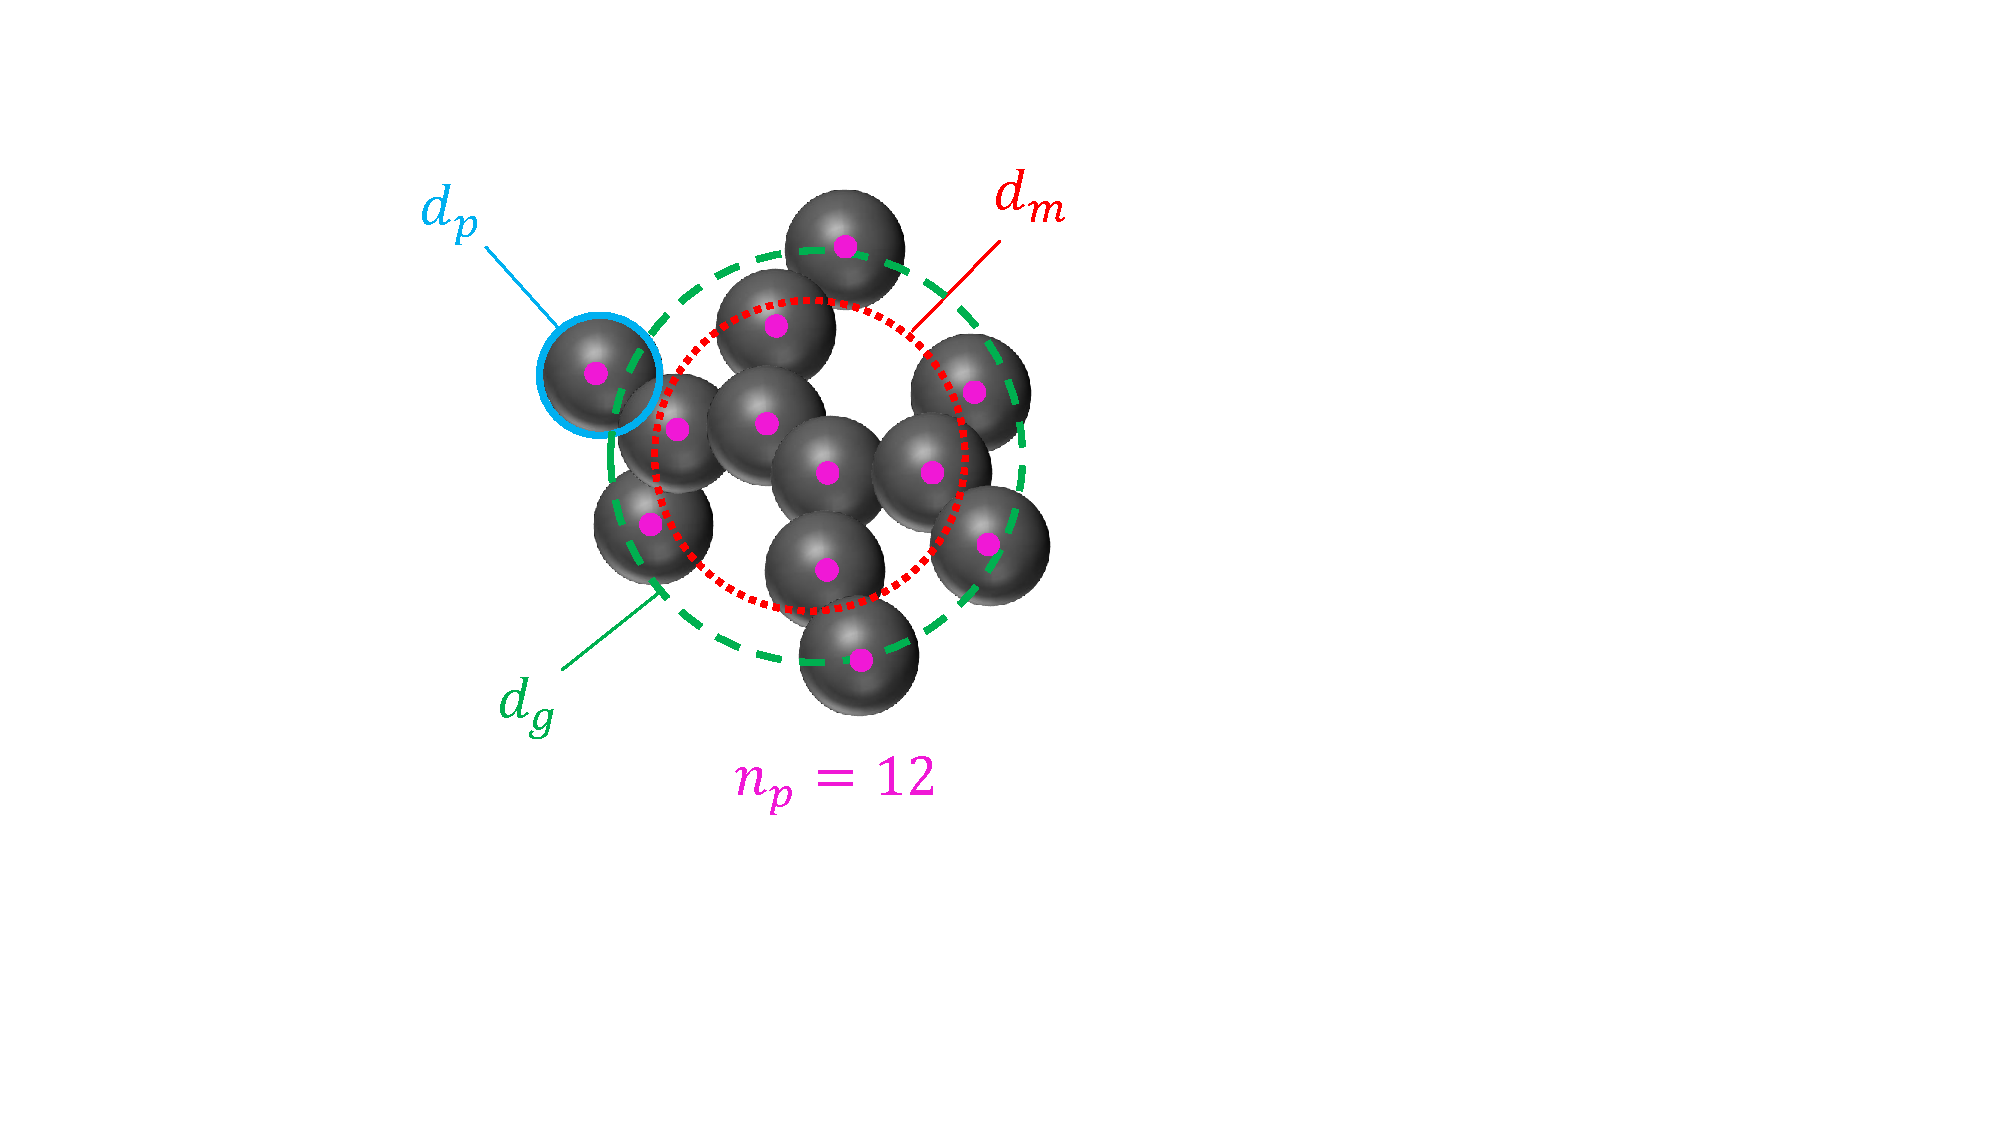
\includegraphics[height=60mm, ]{Figures/Morphology.pdf}
	\caption{The schematics of a soot agglomerates with 12 primary particles (${n_p=12}$). Primary particle (${d_p}$), mobility (${d_m}$), and gyration (${d_g}$) are shown.}
	\label{fig:Morphology}
\end{figure} 

$\mathrm{n^i_p}$ is the number of primary particles per agglomerate for $\mathrm{i^{th}}$ section that can be obtained by dividing the number density of primary particles by the the number density of agglomerates of that section as:

\begin{equation}
	n^i_p = \frac{N^i_{pri}}{N^i_{agg}}
	\label{eqn:n_p}.
\end{equation}

Primary particle diameter, $\mathrm{d^i_p}$, can be obtained from total carbon content and number density of primary particles using

\begin{equation}
	d^i_p = \left(\frac{6}{\pi} \frac{C^i_{tot}\cdot W_{carbon}}{\rho_{soot}} \frac{1}{N^i_{pri}\cdot Av} \right)^{1/3}
	\label{eqn:d_p}.
\end{equation}

The DEM-derived power-laws~\citep{Kelesidis2017} relate ${d^i_m}$ and ${d^i_g}$ to ${d^i_p}$ and ${n^i_p}$ as

\begin{equation}
	d^i_{m} = d^i_p\cdot {n^i_p}^{0.45}
	\label{eqn:d_m},
\end{equation}

\begin{equation}
	d^i_g = 
	\left\{
	\begin{array}{lr}
		d^i_m/({n^i_p}^{-0.2}+0.4), & \text{if } n^i_p > 1.5\\
		d^i_m/1.29. & \text{if } n^i_p\leq 1.5
	\end{array}
	\right.
	\label{eqn:d_g}
\end{equation}

The collision diameter, ${d^i_c}$ is the maximum of ${d^i_{m}}$, ${d^i_{g}}$:

\begin{equation}
	d^i_c = \mathrm{max}\left(d^i_m, d^i_g\right)
	\label{eqn:d_c}
\end{equation}

${d^i_{m}}$, ${d^i_{g}}$, ${d^i_{c}}$ are used to calculate the source terms due to the surface growth, oxidation, PAH adsorption and coagulation. The volume equivalent diameter, $d^i_v$, is the diameter of the sphere with the same mass as agglomerate, and it is obtained as:
\begin{equation}
	d^i_v = d^i_p \cdot {n^i_p}^{1/3}
	\label{eqn:d_v}
\end{equation}

The primary particle surface area is calculated from $\mathrm{d^i_p}$ assuming spherical primary particles.
\begin{equation}
	A^i_{p} = \pi {d^i_p}^2
	\label{eqn:Ap},
\end{equation}
$A^i_{tot}$ (for each section) is defined as the total surface area of soot particles per unit mass of gas mixture obtained as
\begin{equation}
	A^i_{tot} = N^i_{pri}\cdot Av\cdot A^i_{p}
	\label{eqn:Atot}.
\end{equation}

\subsection{Diffusion of soot particles}

The diffusion coefficient of soot particle, $D^i$, is calculated as

\begin{equation}
	D^i = \frac{k_B T}{f^i}
	\label{eqn:diff},
\end{equation}
\noindent where $f^i$ is the friction factor of particles in gas,

\begin{equation}
	f^i = \frac{3\pi\mu d^i_m}{C^i(d^i_m)}
	\label{eqn:fraction},
\end{equation}

\noindent where ${C^i}$ is the Cunningham function that corrects the friction factor given a diameter in the continuum regime for transition and free molecular regimes as: 
\begin{equation}
	C^i(d) = 1+\frac{2\lambda}{d}
	\left(
	1.21+0.4\cdot\mathrm{exp}(\frac{-0.78d}{\lambda})
	\right)
	\label{eqn:cun},
\end{equation}
\noindent where $\lambda$ is the mean free path of gas given as:
\begin{equation}
	\lambda = \frac{\mu}{\rho}\sqrt{\frac{\pi W_{gas}}{2k_B Av T}}
	\label{eqn:lambda}.
\end{equation}
Note that, $\lambda$ is a property of the gas mixture that does not depend on particle morphology and size section. The mean velocity, ${c^i}$ and mean stop distance of particles, ${\lambda^i_a}$ can be calculated as:

\begin{equation}
	c^i = \sqrt{\frac{8k_B T}{\pi m^i_{agg}}}
	\label{eqn:meanvel}.
\end{equation}

\begin{equation}
	\lambda_a = \frac{8D^i}{\pi c^i}
	\label{eqn:stopdist}.
\end{equation}

The mean distance of particles are also calculated as:
\begin{equation}
	\delta^i_a=\frac{1}{d^i_c\lambda^i_a}
	\left[
		\left(
			d^i_c+\lambda^i_a
		\right)^3
		-\left(
			{d^i_c}^2+{\lambda^i_a}^2
		\right)^{3 / 2}
	\right]
	-d_{c, j}    
	\label{eqn:meandist}.
\end{equation}

\subsection{Soot Composition}
The composition of soot is characterized by their elemental carbon to hydrogen ratio (C/H) is a measure of soot maturity and increases from $\mathrm{C/H<2}$ for incipient soot~\citep{ciajolo1998spectroscopic} to $\mathrm{2<C/H<10}$ for nascent soot~\citep{betrancourt2017investigation} and $\mathrm{C/H>20}$ for mature soot~\citep{michelsen2017probing}. The soot agglomerates are assumed to have pure carbon graphitic core~\citep{kholghy2016core} with all hydrogen atoms on the surface~\citep{blanquart2009analyzing}. C/H ratio can be obtained from total carbon and hydrogen content as:

\begin{equation}
	\left(
		\frac{C}{H}
	\right)^i
	=\frac{C^i_{tot}}{H^i_{tot}}   
	\label{eqn:CtoH}.
\end{equation}

The carbon content of each agglomerate is a predefined parameter in the SPBM (depending on the section the agglomerate is placed), but it can be calculated from dividing ${C_{tot}}$ by ${N_{agg}}$ for the MPBM. The hydrogen content of each agglomerate is calculated for both particle dynamics models as:

\begin{equation}
	H^i_{agg}
	=\frac{H^i_{tot}}{N^i_{agg}}   
	\label{eqn:Hagg}.
\end{equation}


\subsection{Monodisperse Population Balance Model}
The MPBM used in this research tracks the number density of primary particles (N\textsubscript{pri}) and agglomerates (N\textsubscript{agg}), total carbon (C\textsubscript{tot}) and hydrogen (H\textsubscript{tot}) content of soot particles per unit mass of gas mixture. The morphological parameters such as primary particle, mobility and gyration diameters obtained from these soot variables are the average values for the population.

\subsubsection{Coagulation}
\label{sec:monocoag}
Coagulation is the process during which solid and hard soot particles collide and attach at point of contact leading to larger agglomerates. This process conserves the soot mass and composition and number density of primary particles, so coagulation only affects $\mathrm{N_{agg}}$. $\mathrm{I^N_{coag}}$ accounts for the decay rate of $\mathrm{N_{agg}}$ by the binary collision of soot particles by
\begin{equation}
	I_{coag} = -\frac{1}{2}\beta N^2_{agg}
	\label{eqn:Icoag},
\end{equation}
where $\mathrm{\beta}$ is the collision frequency of agglomerates for the free molecular ($\mathrm{Kn>10}$) to continuum regime ($\mathrm{Kn<0.1}$). The value of $\mathrm{\beta}$ in the transition regime ($\mathrm{0.1<Kn<10}$) can be calculated from the harmonic mean of the continuum ($\mathrm{\beta_{cont}}$) and free molecular ($\mathrm{\beta_{fm}}$) regime values. Additionally, an enhancement factor of \%82 is applied to take into account the effect of polydispersity~\citep{kelesidis2021self} as:
\begin{equation}
	\beta = 1.82\frac{\beta_{fm}\beta_{cont}}{\beta_{fm}+\beta_{cont}}
	\label{eqn:betahmmono},
\end{equation}
\begin{equation}
	\beta_{fm} = 4\sqrt{\frac{\pi k_b T}{m_{agg}}} d^2_c
	\label{eqn:betafmmono},
\end{equation}
\begin{equation}
	\beta_{cont} = 8\pi d_c D
	\label{eqn:betacontmono}.
\end{equation}

Alternatively, $\mathrm{\beta}$ can be obtained using Fuchs interpolation~\citep{fuchs1965mechanics} as:

\begin{equation}
	\beta = \beta_{cont}
	\left(
		\frac{d_c}{d_c+2\sqrt{2}\delta} +
		\frac{8D}{\sqrt{2}c_r d_c}
	\right)^{-1}
	\label{eqn:betafuchsmono}.
\end{equation}

\subsubsection{Source terms}
The source terms of tracked variables combines the effect of the inception, PAH adsorption, surface growth and oxidation and coagulation.

\begin{equation}
	S_{N_{agg}} = \frac{I_{N,inc}}{n_{c,min}}+I_{coag}
	\label{eqn:S_N_agg}.
\end{equation}
\begin{equation}
	S_{N_{pri}} = \frac{I_{N,inc}}{n_{c,min}}
	\label{eqn:S_N_pri}.
\end{equation}
\begin{equation}
	S_{C_{tot}} = I_{C_{tot},inc}+I_{C_{tot},gr}+I_{C_{tot},ads}+I_{C_{tot},ox}
	\label{eqn:S_C_tot}.
\end{equation}
\begin{equation}
	S_{H_{tot}} = I_{H_{tot},inc}+I_{H_{tot},gr}+I_{H_{tot},ads}+I_{H_{tot},ox}
	\label{eqn:S_H_tot}.
\end{equation}
The partial source terms in Equations~\ref{eqn:S_N_agg}-\ref{eqn:S_H_tot} denoted by $\mathrm{I}$ are determined by PAH growth and surface reaction model explained in Sections~\ref{sec:pahgrowmodel} and~\ref{sec:surfreacmodel}, respectively.

\subsection{Sectional Population Balance Model}
A SPBM with the fixed pivot is used to describe particle dynamics~\citep{wu1988discrete}. The mass range of particles are divided into discrete sections each of which includes agglomerates of the same mass. Inception introduces new particles to the first section with the mass corresponding to the incipient particle. The particles of first section can migrate to upper sections by gaining mass via surface growth and coagulation, and return to lower sections when they lose mass through oxidation. The mass of sections is determined by a geometric progression with a scale factor equal to the mass of incipient soot particle, and a common ratio of SF, known as sectional spacing factor. The mass of each section is approximated by the carbon content of agglomerates in moles as:
\begin{equation}
	C^i_{agg} = \frac{n_{c,min}}{Av}\cdot SF^{(i-1)}
	\label{eqn:Caggsec}.
\end{equation}
\noindent where (i-1) represents the exponent of SF. The mass of hydrogen is ignored in the placement of agglomerates in the sections.
The total number density of agglomerates, $\mathrm{N^i_{agg} [mol/kg]}$, and primary particles, $\mathrm{N^i_{pri} [mol/kg]}$ are tracked for each section. Morphological parameters are determined for each section according to the equations in Section~\ref{sec:sootmorphology}.

\begin{figure}[!htbp]
	\centering
	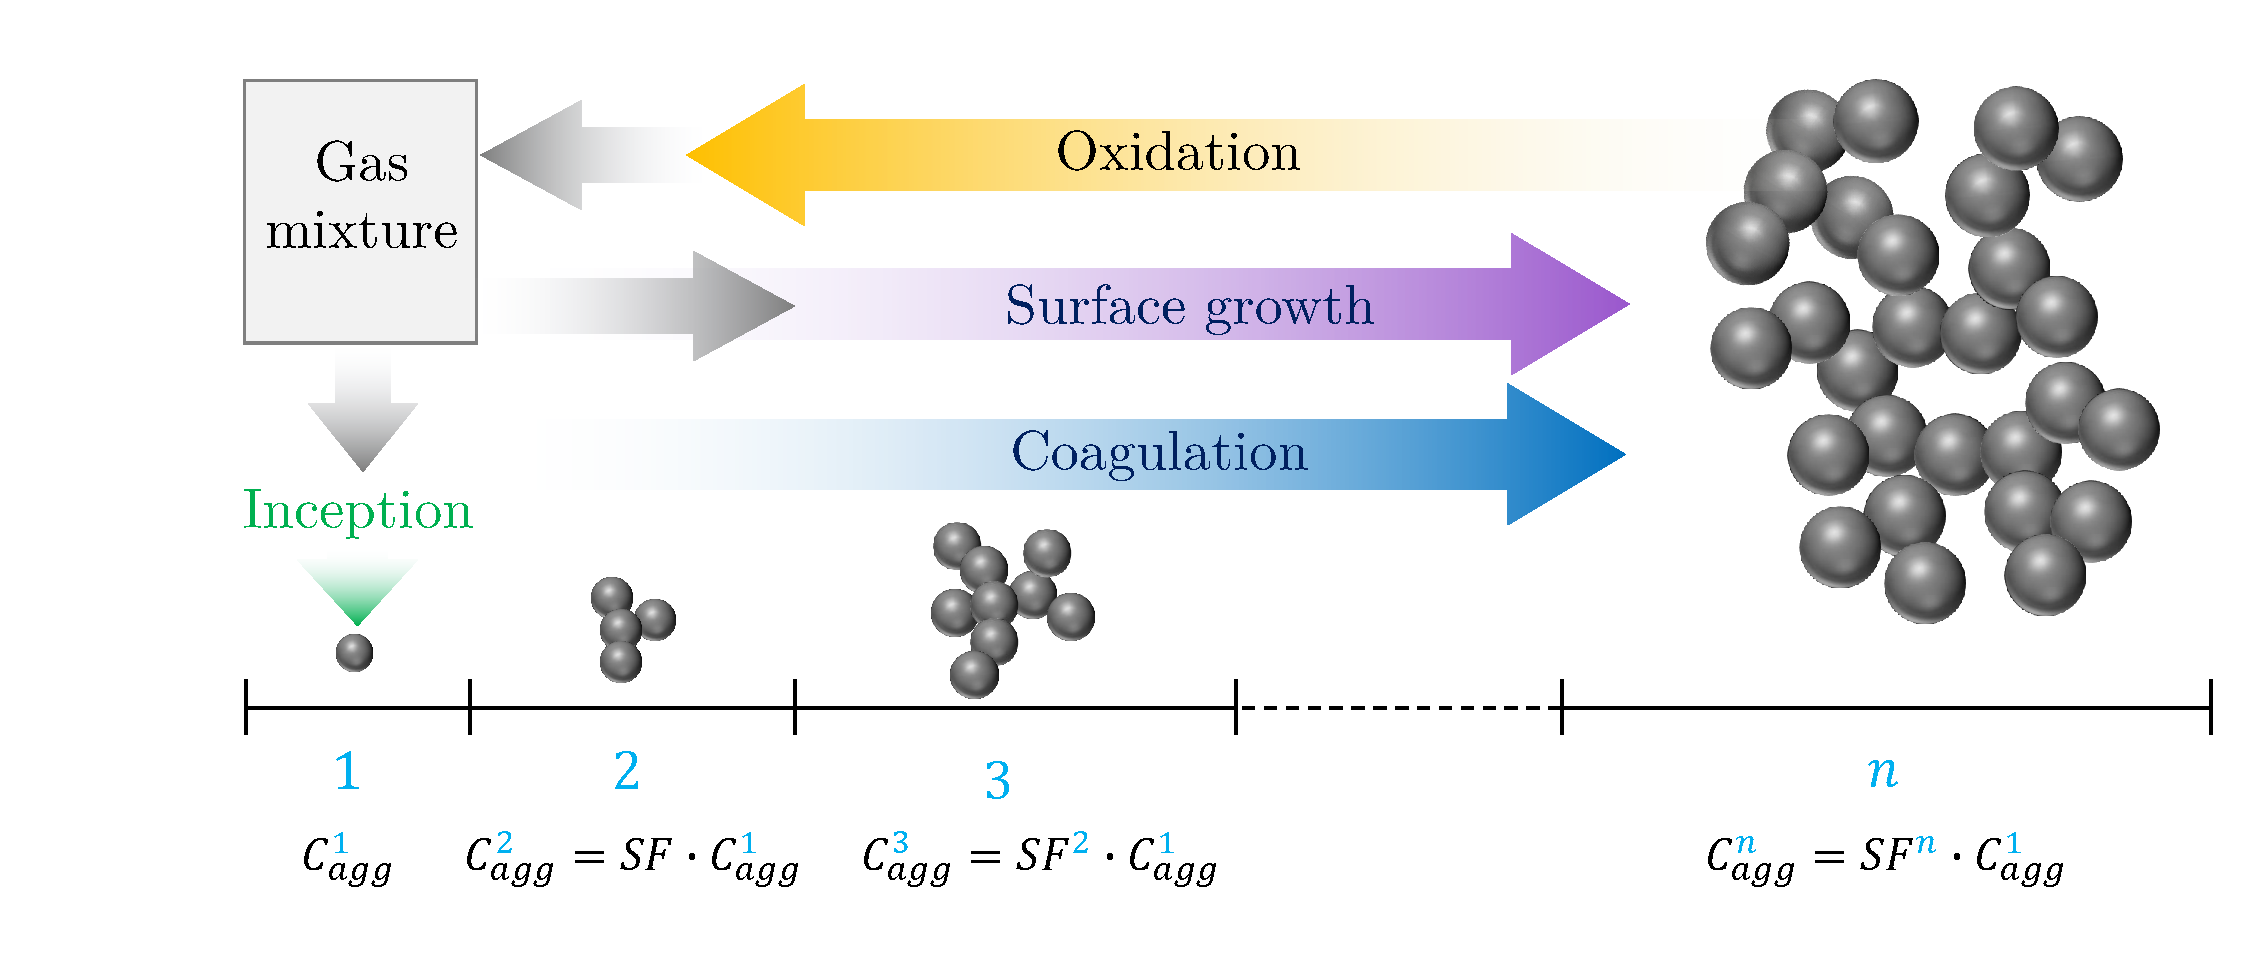
\includegraphics[height=40mm, ]{Figures/Theory/Sectional.pdf}
	\caption{The illustration of sections of SPBM. The mass of sections grows progressively by the scale factor of SF. Inception introduces new particles to the first section that propagate to the upper section via coagulation and surface growth and return to lower sections by oxidation. Carbon and hydrogen pass from gas to solid phase through inception and surface growth and goes back via oxidation.}
	\label{fig:sectional}
\end{figure}

\subsubsection{Coagulation}
\label{sec:sectcoag}
In SPBM approach, collisions between particles from every two sections are considered. The new particles formed by coagulation are placed in a upper section with the mass equal to sum of mass of particles involved in the collision. When the mass of yielded particle lies between two consecutive sections, the particles are divided among these sections proportional to their mass. One possible scenario is that the mass of the newly formed particle is greater than the last section, thus leaving tracked mass range. Losing mass is a potential problem with the fixed pivot sectional model, which can be avoided by selecting proper number of sections and spacing factor to ensure the last sections stay empty during the simulation.

The collision frequency between sections j and k can be obtained from the harmonic mean of the values in the continuum and free molecular regimes as:

\begin{equation}
	\beta^{jk} = 				       \frac{\beta^{jk}_{fm}\beta^{jk}_{cont}}{\beta^{jk}_{fm}
		+\beta^{jk}_{cont}}
	\label{eqn:betahmsect},
\end{equation}

\begin{equation}
	\beta^{jk}_{fm} =
	\sqrt{
		\frac{\pi k_b T}{2}
		\left(
			\frac{1}{m^j_{agg}}+
			\frac{1}{m^k_{agg}}
		\right)
	} 
	\left(
		d^j_c+d^k_c
	\right)^2
	\label{eqn:betafmsect},
\end{equation}
\begin{equation}
	\beta^{ij}_{cont} = \frac{2k_BT}{3\mu}
	\left(
		\frac{C^j}{d^j_m}+
		\frac{C^k}{d^k_m}
	\right)
	\left(
		d^j_c+d^k_c
	\right)^2
	\label{eqn:betacontsect}.
\end{equation}

The collision frequency can also be determined from the Fuchs interpolation similar to the MPBM as:

\begin{equation}
	\beta^{jk}=
	\beta^{ij}_{cont}
	\left[
		\frac{d^j_c+d^k_c}{d^j_c+d^k_c+2+\delta^{jk}_r}+
		\frac{8\left(D^j+D^k\right)}
		{\bar{c}^{jk}_r\left(d^j_c+d^k_c\right)}
	\right]^{-1}
	\label{eqn:betafuchssect},
\end{equation}
\noindent where ${\delta^{jk}_r}$ and ${\bar{c}^{jk}_r}$ are the mean square root of mean distance and velocity of particles, respectively.

\begin{equation}
 	\delta^{jk}_r=
	\sqrt{
		{\delta^j_a}^2+{\delta^k_a}^2
	}
 	\label{eqn:sqrtmeandist},
\end{equation}

\begin{equation}
	\bar{c}^{jk}_r=
	\sqrt{
		{c^j}^2+{c^k}^2
	}
	\label{eqn:sqrtmeanvel}.
\end{equation}

Coagulation redistributes the total number of agglomerates and primary particles as well as hydrogen atoms among the sections. The partial coagulation source terms for ${N^i_{agg}}$, ${N^i_{pri}}$ and ${H^i_{tot}}$ can be calculated as:

\begin{equation}
	I^i_{N_{agg}}
	=
	\sum_{k=1}^{n_{sec}}\sum_{j=k}^{n_{sec}}
	\left(
		1-\frac{\delta_{jk}}{2}
	\right)
	\eta_{ijk}\beta^{jk}N^j_{agg}N^k_{agg}
	-
	N^i_{agg}
	\sum_{k=1}^{n_{sec}}\beta^{im}N^m_{agg}
	\label{eqn:IcoagNaggsect}.
\end{equation}

\begin{equation}
	I^i_{N_{pri}}
	=
	\sum_{k=1}^{n_{sec}}\sum_{j=k}^{n_{sec}}
	\left(
	1-\frac{\delta_{jk}}{2}
	\right)
	\eta_{p,ijk}\eta_{ijk}\beta^{jk}N^j_{agg}N^k_{agg}
	-
	N^i_{pri}
	\sum_{k=1}^{n_{sec}}\beta^{im}N^m_{agg}
	\label{eqn:IcoagNprisect}.
\end{equation}

\begin{equation}
	I^i_{H_{tot}}
	=
	\sum_{k=1}^{n_{sec}}\sum_{j=k}^{n_{sec}}
	\left(
	1-\frac{\delta_{jk}}{2}
	\right)
	\eta_{h,ijk}\eta_{ijk}\beta^{jk}N^j_{agg}N^k_{agg}
	-
	H^i_{tot}
	\sum_{k=1}^{n_{sec}}\beta^{im}N^m_{agg}
	\label{eqn:IcoagHtotsect}.
\end{equation}
\noindent where ${\delta_{jk}}$ is the Kronecker delta defined as:

\begin{equation}
	\delta_{jk}=
	\left\{
	\begin{array}{lr}
		1, & \text{if } j = k\\
		0. & \text{if } j \neq k
	\end{array}
	\right.
	\label{eqn:deltakronecker}
\end{equation}

In Equation~\eqref{eqn:IcoagNaggsect}, $\mathrm{\eta_{ijk}}$ assigns newly formed agglomerates to the two consecutive sections in order to conserve mass during coagulation~\citep{park2005aerosol}.

\begin{equation}
	\eta_{ijk}=
	\left\{
	\begin{aligned}
	&\frac{C^{i+1}_{agg}-C^{jk}_{agg}}{C^{i+1}_{agg}+C^i_{agg}},
	&&
	\text{if } C^i_{agg} \le C^{jk}_{agg} < C^{i+1}_{agg}
	\\
	&\frac{C^{i}_{agg}-C^{jk}_{agg}}{C^{i}_{agg}+C^{i-1}_{agg}}, 
	&&
	\text{if } C^{i-1}_{agg} \le C^{jk}_{agg} < C^{i}_{agg}
	\\
	&0
	&&\text{else}
	\end{aligned}
	\right.
	\label{eqn:etacoag}
\end{equation}
\noindent where ${C^{jk}_{agg}=C^{j}_{agg}+C^{k}_{agg}}$. Similarly, $\eta_{p,ijk}$ in Equation~\eqref{eqn:IcoagNprisect} and $\eta_{h,ijk}$ in Equation~\eqref{eqn:IcoagHtotsect} adjust the number of primary particles and hydrogen atoms added to consecutive sections based on their mass, respectively.

\begin{equation}
	\eta_{p,ijk}=
	\frac{C^i_{agg}}{C^{jk}_{agg}}
	\left(
		n^j_p + n^k_p
	\right)
	\label{eqn:etapcoag},
\end{equation}

\begin{equation}
	\eta_{h,ijk}=
	\frac{C^i_{agg}}{C^{jk}_{agg}}
	\left(
	H^j_{agg} + H^k_{agg}
	\right)
	\label{eqn:etahcoag},
\end{equation}

\subsubsection{Source terms}
The source terms are split into four parts showing the contribution of different soot formation and evolution factors. The effect of surface growth and PAH adsorption are combined (denoted by the subscript gr,ads) because they are similar mass-gaining mechanisms.

\begin{equation}
	S_{N_{agg}} = 
	\left(S_{N_{agg}}\right)_{inc}
	+\left(S_{N_{agg}}\right)_{gr, ads}
	+\left(S_{N_{agg}}\right)_{ox}
	+\left(S_{N_{agg}}\right)_{coag}
	\label{eqn:S_Naggsect},
\end{equation}

\begin{equation}
	S_{N_{pri}} = 
	\left(S_{N_{pri}}\right)_{inc}
	+\left(S_{N_{pri}}\right)_{gr, ads}
	+\left(S_{N_{pri}}\right)_{ox}
	+\left(S_{N_{pri}}\right)_{coag}
	\label{eqn:S_Nprisect},
\end{equation}

\begin{equation}
	S_{H_{tot}} = 
	\left(S_{H_{tot}}\right)_{inc}
	+\left(S_{H_{tot}}\right)_{gr, ads}
	+\left(S_{H_{tot}}\right)_{ox}
	+\left(S_{H_{tot}}\right)_{coag}
	\label{eqn:S_Htotsect}.
\end{equation}

Inception introduces equal number of agglomerates and primary particles to the first section.

\begin{equation}
	\begin{aligned}
	\left(S_{N_{agg}}\right)_{inc} =
	&\frac{1}{Av}\frac{I_{N, inc}}{C^i_{agg}}, && i=1.
	\end{aligned}
	\label{eqn:S_Nagg_incsect}
\end{equation}

\begin{equation}
	\begin{aligned}
	\left(S_{N_{pri}}\right)_{inc} =
	&\frac{1}{Av}\frac{I_{N, inc}}{C^i_{agg}}, && i=1.
	\end{aligned}
	\label{eqn:S_Npri_incsect}
\end{equation}

\begin{equation}
	\begin{aligned}
		\left(S_{H_{tot}}\right)_{inc} =
		&I_{H, inc}, && i=1.
	\end{aligned}
	\label{eqn:S_Htot_incsect}
\end{equation}

Surface growth and PAH adsorption increase the (carbon) mass and hydrogen content of agglomerates, and transfer them to upper sections. The removal rate of agglomerates ($\mathrm{N^i_{agg}}$) from the original section due to surface growth and PAH adsorption must be equal to the addition rate of agglomerates to the target section to conserve the mass, and it is calculated by dividing the mass growth rate by the difference of the mass of the adjacent sections.

\begin{equation}
	\left(S_{N_{agg}}\right)_{gr, ads}=
	\frac{1}{Av}
	\left\{
	\begin{aligned}
		&-\frac{I^i_{C_{tot},gr}+I^i_{C_{tot},ads}}{C^{i+1}_{agg}-C^{i}_{agg}}
		&&
		\text{if } i = 1
		\\
		&\frac{I^{i-1}_{C_{tot},gr}+I^{i-1}_{C_{tot},ads}}{C^{i}_{agg}-C^{i-1}_{agg}}
		-\frac{I^{i}_{C_{tot},gr}+I^{i}_{C_{tot},ads}}{C^{i+1}_{agg}-C^{i}_{agg}}
		&&
		\text{if } 1 < i < n_{sec}
		\\
		&\frac{I^{i-1}_{C_{tot},gr}+I^{i-1}_{C_{tot},ads}}{C^{i}_{agg}-C^{i-1}_{agg}}
		&&\text{if } i=n_{sec}
	\end{aligned}
	\right.
	\label{eqn:S_Nagg_gradssect}
\end{equation}

As agglomerates move up/down through sections, they carry the number of primary particles as well as hydrogen atoms, so the transfer rate of agglomerates is multiplied by $\mathrm{n^i_p}$ and $\mathrm{H^i_{agg}}$, respectively. 

\begin{equation}
	\left(S_{N_{pri}}\right)_{gr, ads}=
	\frac{1}{Av}
	\left\{
	\begin{aligned}
		&-\frac{I^i_{C_{tot},gr}+I^i_{C_{tot},ads}}{C^{i+1}_{agg}-C^{i}_{agg}}
		&&
		\text{if } i = 1
		\\
		&\frac{I^{i-1}_{C_{tot},gr}+I^{i-1}_{C_{tot},ads}}{C^{i}_{agg}-C^{i-1}_{agg}}n^{i-1}_p
		-\frac{I^{i}_{C_{tot},gr}+I^{i}_{C_{tot},ads}}{C^{i+1}_{agg}-C^{i}_{agg}}n^{i}_p
		&&
		\text{if } 1 < i < n_{sec}
		\\
		&\frac{I^{i-1}_{C_{tot},gr}+I^{i-1}_{C_{tot},ads}}{C^{i}_{agg}-C^{i-1}_{agg}}n^{i-1}_p
		&&\text{if } i=n_{sec}
	\end{aligned}
	\right.
	\label{eqn:S_Npri_gradssect}
\end{equation}

\begin{equation}
	\left(S_{H_{tot}}\right)_{gr, ads}=
	\frac{1}{Av}
	\left\{
	\begin{aligned}
		&-\frac{I^i_{C_{tot},gr}+I^i_{C_{tot},ads}}{C^{i+1}_{agg}-C^{i}_{agg}}H^{i}_{agg} 
		+ I^{i}_{H_{tot}, gr} + I^{i}_{H_{tot}, ads}
		&&
		\text{if } i = 1
		\\
		&\frac{I^{i-1}_{C_{tot},gr}+I^{i-1}_{C_{tot},ads}}{C^{i}_{agg}-C^{i-1}_{agg}}H^{i-1}_{agg}
		-\frac{I^{i}_{C_{tot},gr}+I^{i}_{C_{tot},ads}}{C^{i+1}_{agg}-C^{i}_{agg}}H^{i}_{agg}
		+ I^{i}_{H_{tot}, gr} + I^{i}_{H_{tot}, ads}
		&&
		\text{if } 1 < i < n_{sec}
		\\
		&\frac{I^{i-1}_{C_{tot},gr}+I^{i-1}_{C_{tot},ads}}{C^{i}_{agg}-C^{i-1}_{agg}}H^{i-1}_{agg}
		+ I^{i}_{H_{tot}, gr} + I^{i}_{H_{tot}, ads}
		&&\text{if } i=n_{sec}
	\end{aligned}
	\right.
	\label{eqn:S_Htot_gradssect}
\end{equation}

Similarly, the agglomerates lose (carbon) mass by oxidation, and descend to the lower sections carrying primary particle and hydrogen.

\begin{equation}
	\left(S_{N_{agg}}\right)_{ox}=
	\frac{1}{Av}
	\left\{
	\begin{aligned}
		&\frac{I^{i+1}_{C_{tot},ox}}{C^{i+1}_{agg}-C^{i}_{agg}}
		-
		\frac{I^{i}_{C_{tot},ox}}{C^{i}_{agg}}
		&&
		\text{if } i = 1
		\\
		&\frac{I^{i+1}_{C_{tot},ox}}{C^{i+1}_{agg}-C^{i}_{agg}}
		-
		\frac{I^{i}_{C_{tot},ox}}{C^{i}_{agg}-C^{i-1}_{agg}}
		&&
		\text{if } 1 < i < n_{sec}
		\\
		&
		-
		\frac{I^{i}_{C_{tot},ox}}{C^{i}_{agg}-C^{i-1}_{agg}}
		&&\text{if } i=n_{sec}
	\end{aligned}
	\right.
	\label{eqn:S_Nagg_oxsect}
\end{equation}

\begin{equation}
	\left(S_{N_{pri}}\right)_{ox}=
	\frac{1}{Av}
	\left\{
	\begin{aligned}
		&\frac{I^{i+1}_{C_{tot},ox}}{C^{i+1}_{agg}-C^{i}_{agg}}n^{i+1}_p
		-
		\frac{I^{i}_{C_{tot},ox}}{C^{i}_{agg}}
		&&
		\text{if } i = 1
		\\
		&\frac{I^{i+1}_{C_{tot},ox}}{C^{i+1}_{agg}-C^{i}_{agg}}n^{i+1}_p
		-
		\frac{I^{i}_{C_{tot},ox}}{C^{i}_{agg}-C^{i-1}_{agg}}n^{i}_p
		&&
		\text{if } 1 < i < n_{sec}
		\\
		&
		-
		\frac{I^{i}_{C_{tot},ox}}{C^{i}_{agg}-C^{i-1}_{agg}}n^{i}_p
		&&\text{if } i=n_{sec}
	\end{aligned}
	\right.
	\label{eqn:S_Npri_oxsect}
\end{equation}

\begin{equation}
	\left(S_{H_{tot}}\right)_{ox}=
	\frac{1}{Av}
	\left\{
	\begin{aligned}
		&\frac{I^{i+1}_{C_{tot},ox}}{C^{i+1}_{agg}-C^{i}_{agg}}H^{i+1}_{agg}
		-
		\frac{I^{i}_{C_{tot},ox}}{C^{i}_{agg}}H^{i}_{agg}
		+ I^{i}_{H_{tot}, ox}
		&&
		\text{if } i = 1
		\\
		&\frac{I^{i+1}_{C_{tot},ox}}{C^{i+1}_{agg}-C^{i}_{agg}}H^{i+1}_{agg}
		-
		\frac{I^{i}_{C_{tot},ox}}{C^{i}_{agg}-C^{i-1}_{agg}}H^{i}_{agg}
		+ I^{i}_{H_{tot}, ox}
		&&
		\text{if } 1 < i < n_{sec}
		\\
		&
		-
		\frac{I^{i}_{C_{tot},ox}}{C^{i}_{agg}-C^{i-1}_{agg}}H^{i}_{agg}
		+ I^{i}_{H_{tot}, ox}
		&&\text{if } i=n_{sec}
	\end{aligned}
	\right.
	\label{eqn:S_Htot_oxsect}
\end{equation}

\section{Surface reactions model}
\label{sec:surfreacmodel}
The heterogeneous surface reactions are described by hydrogen-abstraction-acetylene-addition (HACA) mechanism~\citep{frenklach1991detailed, appel2000kinetic}. The soot growth in HACA scheme is based on a sequential process similar to PAH growth. The hydrogenated arm-chair sites ($\mathrm{C_{soot}-H}$) on the edge of aromatic rings are dehydrogenated by H abstraction forming $\mathrm{C_{soot\mbox{\textdegree}}}$ that bonds with $\mathrm{C_2H_2}$ resulting in an additional aromatic ring with hydrogenated site. These sites can also be attacked by $\mathrm{O_2}$ or $\mathrm{OH}$. The elementary reactions that describe this sequential process are listed in Table~\ref{tab:HACA}.
The rate of mass growth by HACA is obtained from the reaction of $\mathrm{C_2H_2}$ with dehydrogenated sites as:

\begin{equation}
	\omega^i_{gr} = \alpha^i k_{f4} [\mathrm{C_2H_2}][\mathrm{C_{soot\mbox{\textdegree}}}]
	\label{eqn:hacaRate}.
\end{equation}

\noindent where ${k_{f4}}$ denotes the forward rate of Reaction~\ref{reac:haca4} in Table~\ref{tab:HACA}, and $\mathrm{[C^i_{soot\mbox{\textdegree}}]}$ is obtained by multiplying the surface density of dehydrogenated sites, $\mathrm{\chi_{soot\mbox{\textdegree}}}$ with total surface area of soot (per unit of mass of gas mixture) as:

\begin{equation}
	[\mathrm{C^i_{soot\mbox{\textdegree}}}] = \frac{\rho}{Av}A^i_{tot}\cdot\chi_{soot\mbox{\textdegree}}
	\label{eqn:csoot0}.
\end{equation}

$\mathrm{\chi_{soot\mbox{\textdegree}}}$ is calculated by assuming the steady-state for $\mathrm{[C_{soot\mbox{\textdegree}}]}$ in the system of reactions in Table~\ref{tab:HACA}:
\begin{equation}
	\chi_{soot\mbox{\textdegree}} = 
	\frac
	{k_{f1}[\mathrm{H}]+k_{f2}[\mathrm{OH}]}
	{k_{r1}[\mathrm{H_2}]+k_{r2}[\mathrm{H_2O}]+k_{f3}[\mathrm{H}]+k_{f4}[\mathrm{C_2H_2}]+k_{f5}[\mathrm{O_2}]+k_{f1}[\mathrm{H}]+k_{f2}[\mathrm{OH}]} \chi_{soot_{CH}}
	\label{eqn:chisoot0},
\end{equation}
\noindent where $\mathrm{\chi_{soot_{CH}}}$ is the surface density of hydrogenated sites estimated based on the assumption that soot surface is covered with stacks of benzene rings~\citep{appel2000kinetic}. Considering the stack spacing of 3.15$\mathrm{\AA}$ and 2 C–H bonds per benzene ring length, the surface density of hydrogenated sites, $\chi_{{soot}-H}$, is calculated to be $0.23\:\mathrm{site/\AA^2}=2.3\times10^{19} \mathrm{site/m^2}$, which gives the maximum theoretical limit of the reaction sites.

In Equation~\eqref{eqn:hacaRate}, $\alpha$ is the surface reactivity factor between 0 and 1 that represents the decline of reaction sites from the theoretical limit due to particle aging, growth and maturity~\citep{haynes1982surface, harris1985chemical}, and it has been observed to depend on temperature time history~\cite{homann1985formation, dasch1985decay}. The value of $\alpha$ has been described using constant target-specific values as well as empirical equations based on particle size and flame temperature. A detailed review of these can be found in the chapter 4 of \citep{veshkini2015understanding}.  Here, the empirical equations proposed by \citet{appel2000kinetic} is used to calculate $\mathrm{\alpha}$:
\begin{equation}
	\alpha^i = \tanh 
	\left(
	\frac{12.56 - 0.00563\cdot T}
	{\mbox{log}_{10}
		\left( \frac{\rho_{soot}\cdot Av}{W_{carbon}} \frac{\pi}{6}{d^i_p}^3 \right) } -1.38+0.00068\cdot T
	\right)
	\label{eqn:alpha}.
\end{equation}

Alternatively, \citet{blanquart2009joint} related $\mathrm{\alpha}$ to the number of surface hydrogen atoms on the soot particles.

\begin{equation}
	\alpha^i = \frac{H^i_{tot}}{C^i_{tot}}
	\label{eqn:alpha_htoc}.
\end{equation}

The contribution of HACA to growth source terms can be computed from HACA rates considering the number of carbon atoms in $\mathrm{C_2H_2}$ and number of arm-chair and zig-zag hydrogenated sites on soot particle~\cite{blanquart2009analyzing} using

\begin{equation}
	I^i_{C_{tot},gr} = 2\omega^i_{gr}/\rho
	\label{eqn:IiCtotgr},
\end{equation}
\begin{equation}
	I^i_{H_{tot},gr} = 0.25\omega^i_{gr}/\rho
	\label{eqn:IiHtotgr}.
\end{equation}

The rate change of $\mathrm{C_2H_2}$ concentration due to mass growth is written as:

\begin{equation}
	\left(\frac{d\left[{\mathrm{C_2H_2}}\right]}{dt}\right)_{gr} = -\sum_{i=1}^{n_{sec}}\omega^i_{gr}
	\label{eqn:C2H2rate_gr}.
\end{equation}

The rate of release of H radicals into the gas mixture due to surface growth is:

\begin{equation}
	\left(\frac{d\left[{\mathrm{H}}\right]}{dt}\right)_{gr} = 1.75 \sum_{i=1}^{n_{sec}}\omega^i_{gr}
	\label{eqn:Hrate_gr}.
\end{equation}

\renewcommand{\arraystretch}{1.5}
\begin{table}
	\caption{Rate coefficients for the various surface reactions in Arrhenius form $\mathrm{k=AT^n\cdot e^{-E/RT}}$}
	\label{tab:HACA}
	\centering
	\begin{tabular}{l l l l l l}
		\hline
		No. & Reaction & \hspace{0.1cm} & A~$\mathrm{\left[ \frac{m^3}{mol\cdot s} \right]}$ & n & $\mathrm{\frac{E}{R} [K]}$  \\
		\hline
		\stepcounter{reaction}\thetag{\thereaction}\label{reac:haca1} & \ce{C_{soot-H} + H <--> C_{soot\textdegree} + H_2}  & f & $4.17\times 10^7$ & 0 & 6542.52 \\
		& & r & $3.9\times 10^6$ & 0 & 5535.98 \\
		\stepcounter{reaction}\thetag{\thereaction}\label{reac:haca2} & \ce{C_{soot-H} + OH <--> C_{soot\textdegree} + H_2O} & f & $10^4$ & 0.734 & 719.68\\
		&  & r & 3.68$\times 10^2$ & 1.139 & 8605.94 \\
		\stepcounter{reaction}\thetag{\thereaction}\label{reac:haca3} & \ce{C_{soot\textdegree} + H -> C_{soot} + H_2O} & f & $10^4$ & 0.734 & 719.68\\
		\stepcounter{reaction}\thetag{\thereaction}\label{reac:haca4} & \ce{C_{soot\textdegree} + C_2H_2 -> C_{soot-H}} & f & 80 & 1.56 & 1912.43\\
		\stepcounter{reaction}\thetag{\thereaction}\label{reac:haca5} & \ce{C_{soot\textdegree} + O_2 -> 2CO} & f & 2.2 $\times 10^6$ & 0 & 3774.53\\
		\stepcounter{reaction}\thetag{\thereaction}\label{reac:haca6} & \ce{C_{soot}-H + OH -> CO + \frac{1}{2} H_2} & f & $1.3\times 10^7$ & 0 & 0\\
		\hline
	\end{tabular}
\end{table}


The carbons on the surface of soot are oxidized via reaction with $\mathrm{O_2}$ and $\mathrm{OH}$ which decreases total carbon of soot and releases CO and $\mathrm{H_2}$ to gas mixture. The oxidation process is described by HACA mechanism. $\mathrm{O_2}$ and $\mathrm{OH}$ oxidation rates are calculated as

\begin{equation}
	\omega^i_{ox,O_2} = \alpha^i k_{f5} [\mathrm{O_2}][C^i_{soot\mbox{\textdegree}}]
	\label{eqn:hacaO2Rate},
\end{equation}

\begin{equation}
	\omega^i_{ox,OH} = \alpha^i k_{f6} [\mathrm{OH}][soot^i]
	\label{eqn:hacaOHRate}.
\end{equation}

The oxidation source term is calculated considering the number of carbon atoms removed from soot through each oxidation pathway by

\begin{equation}
	I^i_{C_{tot},ox} = -(2\omega^i_{ox,O_2} + \omega^i_{ox,OH})/\rho
	\label{eqn:ICtot},
\end{equation}

We assume that oxidation does not change the number of surface hydrogen atoms. The rate change of concentration of CO, H and OH by oxidation is calculates as:

\begin{equation}
	\left(\frac{d\left[{\mathrm{CO}}\right]}{dt}\right)_{ox} = \sum_{i=1}^{n_{sec}}\omega^i_{ox,O_2}
	\label{eqn:COrate_ox}.
\end{equation}

\begin{equation}
	\left(\frac{d\left[{\mathrm{O_2}}\right]}{dt}\right)_{ox} = -\sum_{i=1}^{n_{sec}}\omega^i_{ox,O_2}
	\label{eqn:COrate_ox}.
\end{equation}

\begin{equation}
	\left(\frac{d\left[{\mathrm{OH}}\right]}{dt}\right)_{ox} = -\sum_{i=1}^{n_{sec}}\omega^i_{ox,OH}
	\label{eqn:Hrate_ox}.
\end{equation}

\begin{equation}
	\left(\frac{d\left[{\mathrm{H_2}}\right]}{dt}\right)_{ox} = \frac{1}{2}\sum_{i=1}^{n_{sec}}\omega^i_{ox,OH}
	\label{eqn:OHrate_ox}.
\end{equation}

\section{PAH growth models}
\label{sec:pahgrowmodel}
Here, four different PAH growth models are used to describe the conversion of PAHs to incipient particles and their adsorption on existing agglomerates. As mentioned before, the soot inception and surface growth is not fully understood yet, but there is substantial evidence to support the collision of PAHs as a key step in inception and surface growth~\citep{zhao2003measurement, abid2009quantitative, happold2009soot}. So, global inception models have been developed based PAH collision consisting of different pathways with single- or multi-step reactions. The collision frequency of gaseous species including PAH molecules and polymers depend on their mass and diameter, and it is obtained as:

\begin{equation}
	\beta_{dim_{jk}}=
	2.2 \cdot d^2_{r} \sqrt{\frac{8 \pi k_B T}{m_{r}}}
	\label{eqn:betadim}
\end{equation}

where $\mathrm{d_{r}}$ and $\mathrm{m_{r}}$ are reduced diameter and mass for two PAH molecules, respectively.

\begin{equation}
	d_{r}=
	2\frac{d_{PAH_k}\cdot d_{PAH_j}}{d_{PAH_k}+d_{PAH_k}}
	\label{eqn:drPAH}
\end{equation}

\begin{equation}
	m_{r}=
		\frac{m_{PAH_k}\cdot m_{PAH_k}}{m_{PAH_j}+ m_{PAH_j}}
	\label{eqn:mrPAH}
\end{equation}

The mass of each PAH molecule is obtained from its molecular weight as:

\begin{equation}
	m_{PAH_j}=
	\frac{W_{PAH_j}}{Av}
	\label{eqn:mPAH}
\end{equation}

The diameter of PAH is calculated from its mass and density.

\begin{equation}
	d_{PAH_j}=
	\left(
		\frac{6\cdot m_{PAH_j}}{\pi\cdot\rho_{PAH_j}}
	\right)^{1/3}
	\label{eqn:dPAH}
\end{equation}

The density of a PAH molecule is estimated using the relation proposed by \citet{johansson2016formation}.

\begin{equation}
	\rho_{PAH_j}= 
	171943.5197
	\frac{W_{carbon}\cdot n_{C,PAH_j}+W_{hydrogen}\cdot n_{H,PAH_j}}
	{n_{C,PAH_j}+n_{H,PAH_j}}
	\label{eqn:rhoPAH}
\end{equation}

The collision frequency of $\mathrm{PAH_j}$ and soot agglomerates in each section can be determined for the entire regime by harmonic mean of the collision frequency in the free molecular and continuum regimes as:

\begin{equation}
	\beta^i_{ads_j}=
	\frac{\beta^i_{fm, ads}\cdot \beta^i_{cont, ads}}
	{\beta^i_{fm, ads}+\beta^i_{cont, ads}}
	\label{eqn:betahmads}
\end{equation}

\begin{equation}
	\beta^i_{fm, ads_j}=
	2.2 
	\sqrt{
		\frac{\pi k_B T}{2}\left(\frac{1}{m^i_{agg}}+\frac{1}{m_{PAH_j}}\right)
	}
	\left(d^i_g+d_{PAH}\right)^2
	\label{eqn:betafmads}
\end{equation}

\begin{equation}
	\beta^i_{cont, ad_js}=
		\frac{2 k_B T}{3 \mu}
		\left[
			\frac{C^i\left(d_m\right)}{d^i_g}+
			\frac{C^i\left(d_{PAH_j}\right)}{d_{PAH_j}}
		\right]
		\left(d_g+d_{PAH_j}\right)
	\label{eqn:betacontads}
\end{equation}
where $C^i$ is the Cunningham function calculated by Equation~\ref{eqn:cun}.
\subsection{Irreversible Dimerization}

The irreversible dimerization is based on the irrversible collision of PAHs leading to their clustering/polymerization that forms dimers, trimers, and tetramers until the polymer mass reaches a threshold that can be considered a solid particle. For practical purposes, dimer is usually considered as a incipient particle that grows by surface growth and coagulation. A single-step irreversible collision of two similar PAHs forms a new dimer as:

\reaction[react:irrevdiminc]{
	$\mathrm{PAH_j}$ + $\mathrm{PAH_j}$ ->[k_{f,dim_j}] $\mathrm{Dimer_j}$
}
Similarly, the adsorption of each PAH molecule on soot particles is described by the irreversible collision of soot and $\mathrm{PAH_j}$ as:
\reaction[react:irrevdimads]{
	$\mathrm{PAH_j}$ + Soot ->[k_{f,ads_j}] $\mathrm{Soot-PAH_j}$
}
The forward rate of dimerization, ${k_{f,dim_j}}$ and adsorption, $k_{f,ads_j}$ in Reactions~\eqref{react:irrevdiminc} and \eqref{react:irrevdimads} are calculated from Equations \eqref{eqn:betadim} and \eqref{eqn:betahmads}, respectively.

\begin{equation}
	k_{f,dim_j}=
	\gamma_{inc}\cdot\beta_{jk,PAH}\cdot Av
	\label{eqn:kfdim},
\end{equation}

\begin{equation}
	k^i_{f,ads_j}=
	\gamma_{ads_j}\cdot\beta^i_{j,ads}\cdot Av
	\label{eqn:kfads},
\end{equation}

where $\mathrm{\gamma_{inc}}$ and $\mathrm{\gamma_{ads}}$ are the collision efficiencies for dimerization and adsorption, respectively. Their value vary in the range of [$\mathrm{10^{-7}}$, 1], and are usually chosen to match the predicted soot mass with the experimental data. Here, $\mathrm{\gamma_{inc}}=10^{-4}$ and $\mathrm{\gamma_{ads}=10^{-3}}$. The rate of dimerization and adsorption from $\mathrm{PAH_j}$ are calculated accordingly as:
\begin{equation}
	w_{dim_j} = k_{f,dim_{jj}} [PAH_j] [PAH_j]
\end{equation}

The partial source terms for inception are calculated as:

\begin{equation}
	I_{N,inc} =\frac{1}{\rho} \sum_{j=1}^{n_{PAH}} w_{dim_j} 2n_{PAH_j,C}
	\label{eqn:INinc}
\end{equation}
\begin{equation}
	I_{C_{tot},inc} = \frac{1}{\rho}\sum_{j=1}^{n_{PAH}} w_{dim_j} 2n_{PAH_j,C}
	\label{eqn:ICtotinc}
\end{equation}
\begin{equation}
	I_{H_{tot},inc} =\frac{1}{\rho} \sum_{j=1}^{n_{PAH}} w_{dim_j} 2n_{PAH_j,H}
	\label{eqn:IHtotinc}
\end{equation}
The rate of PAH adsorption for each section is obtained as:
\begin{equation}
	w^i_{ads_j} = k^i_{f,ads_{j}} [\mathrm{soot}] [PAH_j]
	\label{eqn:adsrate_irrevdim}
\end{equation}
The contribution of PAH adsorption to the source terms are expressed as:

\begin{equation}
	I^i_{C_{tot},ads} = \frac{1}{\rho}\sum_{j=1}^{n_{PAH}} w^i_{ads_j} n_{PAH,C}
	\label{eqn:ICtotads}
\end{equation}
\begin{equation}
	I^i_{H_{tot},ads} =\frac{1}{\rho} \sum_{j=1}^{n_{PAH}} w^i_{dim_j} (n_{PAH,H}-2)
	\label{eqn:IHtotads}
\end{equation}


Each PAH molecule loses one H atom becoming a radical that forms bonds with a dehydrogenated site on soot surface, so two H atoms are released during the process that is taken into account in Equation~\eqref{eqn:IHtotads}.

The formation of a dimer consumes two PAH molecules, and during adsorption one PAH molecule is removed from the gas mixture, so the total rate of $\mathrm{PAH_i}$ removal by the irreversible dimerization is obtained as:

\begin{equation}
	\left(
		\frac{d\left[{\mathrm{PAH_j}}\right]}{dt}
	\right)_{inc}
	= 
	-2w_{dim_j}-\sum_{i=1}^{n_{sec}}w^i_{ads_j}
	\label{eqn:PAHscrub_irrevdim}.
\end{equation}

During the adsorption process one $\mathrm{H_2}$ is released to the gas mixture.
\begin{equation}
	\left(
		\frac{d\left[{\mathrm{H_2}}\right]}{dt}
	\right)_{inc}
	= 
	\sum_{i=1}^{n_{sec}}w^i_{ads_j}
	\label{eqn:H2scrub_irrevdim}.
\end{equation}


\subsection{Reactive Dimerization}
This model is built on Irreversible Dimerization with two main differences: The first step of dimerization and adsorption is reversible forming physically bonded dimers followed by a irreversible carbonization that leads to chemical bond formation in dimers \citep{kholghy2018reactive}. This approach allows formation of homo- and heterodimers. The dimerization of $\mathrm{PAH_j}$ and $\mathrm{PAH_k}$ is described as:
\reaction[reac:phydim_reacdim]{
	PAH_j + PAH_k <-->[k_{f,dim_{jk}}][k_{r,dim_{jk}}] Dimer^*_{ij},
}
\reaction[reac:chemdim_reacdim]{
	Dimer^*_{jk} ->[k_{reac}] Dimer_{jk},
}
\noindent where $\mathrm{Dimer^*_{jk}}$ and $\mathrm{Dimer_{jk}}$ physically and chemically bonded dimers, respectively, from $\mathrm{PAH_j}$ and $\mathrm{PAH_k}$. The forward rate of physical dimerization, $\mathrm{k_{f,dim_{jk}}}$ is calculated from Equation~\eqref{eqn:betadim} as:

\begin{equation}
	k_{f,dim_{jk}}=
	p^{''}\cdot\beta_{jk,PAH}\cdot Av
	\label{eqn:kfphydim_reacdim},
\end{equation}

where ${p^{''}}=0.1$ accounts for the probability of PAH-PAH collisions in “FACE” configuration that results in successful vdW bond formation~\citep{miller1984intermolecular}. The reverse rate of physical dimerization, ${k_{r,dim_{jk}}}$ is obtained from the dimerization equilibrium constant~\citep{miller1991kinetics} as:
	
\begin{equation}
	\mathrm{log}_{10}K_{eq}=
	a\frac{\epsilon_{jk}}{RT}+b
	\label{eqn:keq_reacdim},
\end{equation}

\begin{equation}
	k_{r,dim_{jk}} = k_{f,dim_{jk}}10^{-b}e^{-a\epsilon_{jk} ln(10)/(RT)}
	\label{eqn:krphydim_reacdim},
\end{equation}

\begin{equation}
	\epsilon_{jk} = cW_{jk} -d
	\label{eqn:epsilon_reacdim},
\end{equation}

\begin{equation}
	W_{jk} = \frac{W_j\cdot W_k}{W_j+W_k}
	\label{eqn:Wjk_reacdim},
\end{equation}
\noindent where ${a=0.115}$ (obtained from pyrere dimerization data~\cite{sabbah2010exploring}) and b=1.8 \cite{kholghy2018reactive}, c=933420~j/kg, and d=34053~j/mol~\cite{kholghy2018reactive}. 

The rate of chemical bond formation, $\mathrm{k_{reac}}$ is defined in the Arrhenius form~\cite{naseri2022simulating} as
\begin{equation}
	k_{reac} = 5\times10^6\cdot e^{(-96232/RT)}
	\label{eqn:kc_reacdim}.
\end{equation}

Assuming a steady state condition for the physical dimers, $\mathrm{\partial [Dimer^*_{jk}]/\partial t=0}$, the rate of formation of chemically-bonded dimers can be obtained as

\begin{equation}
	\omega_{dim_{jk}} = k_{reac}\frac{k_{f,dim_{jk}}[\mathrm{PAH_j}][\mathrm{PAH_k}]}
	{k_{r,dim_{jk}}+k_{c,dim}}
	\label{eqn:chemdimer_reacdim}.
\end{equation}

The contribution of dimer formation to partial source terms is expressed by looping over all combinations of PAHs as:

\begin{equation}
	I_{N,{inc}} = 
	\frac{1}{\rho}
	\sum_{j=1}^{n_{PAH}} \sum_{k=j}^{n_{PAH}}  \omega_{dim_{kj}} 
	\left(
	n_{PAH_j,C}+n_{PAH_k,C}
	\right)
	\label{eqn:IN_inc},
\end{equation}

\begin{equation}
	I_{C_{tot},{inc}} = 
	\frac{1}{\rho}
	\sum_{j=1}^{n_{PAH}} \sum_{k=j}^{n_{PAH}}  \omega_{dim_{kj}} 
	\left(
	n_{PAH_j,C}+n_{PAH_k,C}
	\right)
	\label{eqn:ICtot_inc},
\end{equation}

\begin{equation}
	I_{H_{tot},{inc}} = 
	\frac{1}{\rho}
	\sum_{j=1}^{n_{PAH}} \sum_{k=j}^{n_{PAH}}  \omega_{dim_{kj}} 
	\left(
	n_{PAH_j,H}+n_{PAH_k,H}
	\right)
	\label{eqn:IHtot_inc},
\end{equation}

Similarly, PAH adsorption is described by a two-step process where the collision of $\mathrm{PAH_j}$ with soot agglomerates leads to physically bonded $\mathrm{Soot-PAH^*}$ that is carbonized and forms chemically-bonded $\mathrm{Soot-PAH}$ added to soot surface.

\reaction[reac:physootPAH_reacdim]{
	PAH_j + Soot <-->[k_{f,ads_j}][k_{r,ads_j}] Soot-PAH^*_j,
}

\reaction[reac:chemsootPAH_reacdim]{
	Soot-PAH^*_j ->[k_{c,ads}] Soot-PAH_j,
}

The forward rate of PAH-soot collision is calculated from Equation~\eqref{eqn:betahmads}, and the reverse rate is determined same as inception (Equation\eqref{eqn:krphydim_reacdim}).

\begin{equation}
	k^i_{f,ads}=\beta^i_{jk,ads}\cdot Av
	\label{eqn:kfads_reacdim},
\end{equation}

\begin{equation}
	k^i_{r,ads}=k^i_{f,ads}\cdot10^{-b}e^{-a\epsilon_{soot,j} \mathrm{ln}(10)/(RT)}
	\label{eqn:krads_reacdim},
\end{equation}

\begin{equation}
	\epsilon_{soot,j} = cW_{soot,j} -d
	\label{eqn:epsilonads_reacdim},
\end{equation}

a, b, c, d values are the same as those used in inception. Computing ${\epsilon_{soot,j}}$ also requires "equivalent soot molecular weight", ${W_{soot}}$ for section i, which is estimated from carbon mass of each agglomerate as:

\begin{equation}
	W^i_{soot}=\frac{C^i_{tot}W_{carbon}}{N^i_{agg}} 
\end{equation}

The rate constant of carbonization of $\mathrm{Soot-PAH^*_j}$ is defined as in the Arrhenius form similar to inception (Equation~\eqref{eqn:kc_reacdim}). The prefactor is adjusted based on matching the numercial PSD~\citep{naseri2022simulating} with measurements in the ethylene pyrolysis in a flow reactor~\cite{araki2021effects}. 

\begin{equation}
	k_{c,dim} = 2\times10^{10}\cdot e^{(-96232/RT)}
	\label{eqn:kcads_reacdim}.
\end{equation}


The total adsorption rate can be calculated assuming a steady-state concentration for physically adsorbed PAH on soot, $\mathrm{\partial{[{Soot-PAH^*}]}/\partial t = 0}$ calculated in a similar way to inception flux (Equation~\eqref{eqn:chemdimer_reacdim}) as\\

\begin{equation}
	\omega^i_{ads_j} = k_{c,ads}\frac{k_{f,ads_j}[\mathrm{Soot}][\mathrm{PAH_j}]}{k_{r,ads_j}+k_{c,ads_j}}
	\label{eqn:wads_reacdim},
\end{equation}

The contribution of PAH adsorption rate to partial source terms can be expressed as:

\begin{equation}
	I^i_{C_{tot},ads} =
	\frac{1}{\rho}
	\sum_{i=1}^{n_{PAH}}
	\omega^i_{ads_j}
	n_{C,PAH_j}
	\label{eqn:ICtotads_reacdim},
\end{equation}

\begin{equation}
	I^i_{C_{tot},ads} =
	\frac{1}{\rho}
	\sum_{i=1}^{n_{PAH}}
	\omega^i_{ads_j}
	\left(n_{H,PAH_j}-2\right)
	\label{eqn:IHtotads_reacdim}.
\end{equation}

The rate of removal of PAH from gas mixture due to adsorption is given as

\begin{equation}
	\left(
	\frac{d\left[{\mathrm{PAH_j}}\right]}{dt}
	\right)_{inc}
	= 
	-\sum_{k=1}^{n_{PAH}}w_{dim_{jk}}-\sum_{i=1}^{n_{sec}}w^i_{ads_j}
	\label{eqn:PAHscrub_reacdim}.
\end{equation}

During the adsorption process one $\mathrm{H_2}$ is released to the gas mixture.
\begin{equation}
	\left(
		\frac{d\left[{\mathrm{H_2}}\right]}{dt}
	\right)_{inc}
	= 
	\sum_{i=1}^{n_{sec}}w^i_{ads_j}
	\label{eqn:H2scrub_reacdim}.
\end{equation}

\subsection{Dimer Coalescence}
Dimer coalescence model is a multi-step irreversible model proposed by \citet{blanquart2009joint} where self-collision of PAH molecules form dimers that are intermediate state between gaseous PAH molecules and solid soot particles. The self-coalescence of dimers forms incipient soot particles. Alternatively, dimers can adsorb on the surface of existing soot particles and contribute to their surface growth. The equations are based on implementation of Dimer Coalescence by \citet{sun2021modelling} for a sectional model.

\reaction[reac:dim_dimcoal]{
	PAH_j + PAH_j ->[k_{dim_{j}}] Dimer_{j},
}
\reaction[reac:chemdim_reacdim]{
	Dimer_{j} + Dimer_{j} ->[k_{inc_j}] Tetramer_{j},
}
\reaction[reac:chemdim_reacdim]{
	Dimer_{j} + Soot ->[k_{ads_j}] Soot-PAH_{j},
}

\noindent where the rate constant of dimerization, $\mathrm{k_{dim_{j}}}$ and inception $\mathrm{k_{inc_{j}}}$ are calculated from collision rate of PAHs in Equation~\eqref{eqn:betahmads}.

\begin{equation}
	k_{dim_{j}}=
	\gamma_{dim_j}\cdot\beta_{jj,PAH}\cdot Av
	\label{eqn:kdim_dimcoal},
\end{equation}

\begin{equation}
	k_{inc_{j}}=
	\beta_{jj,dimer}\cdot Av
	\label{eqn:kinc_dimcoal},
\end{equation}

\noindent where $\mathrm{\gamma_{dim_j}}$ is the dimerization efficiency that is assumed to scale with fourth power of PAH molecular weight~\cite{blanquart2009analyzing} as:

\begin{equation}
	\gamma_{dim_j}=
	C_{N,j}\cdot W_{PAH_j}^4
	\label{eqn:gamma_dimcoal},
\end{equation} 

\citet{blanquart2009joint} estimated the constant ${C_{N,j}}$ by comparing the profiles of several PAH species with experimental measurements in a single premixed benzene flame~\citep{tregrossi1999combustion}, and provided efficiency values for various PAHs that are listed in Table~\ref{tab:gammalist_dimcoal}. The rate of dimer collision is expressed as:

\begin{equation}
	w_{dim_j} = k_{inc_{j}} [\mathrm{Dimer_j}] [\mathrm{Dimer_j}]
	\label{eqn:wdim_dimcoal}
\end{equation}

Similarly, the rate of adsorption of dimers on soot particles is obtained as:

\begin{equation}
	w^i_{ads_j} = k^i_{ads_{j}} [\mathrm{soot}]^i [\mathrm{Dimer_j}]
\end{equation}

Assuming fast dimer consumption leads to the steady-state concentration of dimers that can be determined by solving a quadratic equation as:
\begin{equation}
	a_{inc_j}[\mathrm{dimer}]^2+b_{ads_j}[\mathrm{dimer}]=\omega_{dim,j}
	\label{eqn:quad_dimcoal}
\end{equation}
\begin{equation}
	[\mathrm{Dimer_j}]=
	\left\{
	\begin{aligned}
		&\frac{-b_{ads_j}+\sqrt{\Delta_j}}{2a_{inc_j}},
		&&
		\text{if } \Delta_j \ge 0
		\\
		& 0 
		&&
		\text{if } \Delta_j < 0
	\end{aligned}
	\right.
	\label{eqn:dimer_dimcoal}
\end{equation}
\begin{equation}
	\Delta_j = b_{ads_j}^2-4a_{inc_j}\omega_{dim,j}
	\label{eqn:delta_dimcoal}
\end{equation}

where ${a_{inc_j} = k_{inc_{j}}}$ and ${b_{ads_j}}$ is calculated by summing the adsorption rate of dimer for all sections and dividing it by the dimer concentration.

\begin{equation}
	\mathrm{b_{ads_j}} = \sum_{i=1}^{n_sec} k^i_{ads_{j}} [\mathrm{soot}]^i
\end{equation}

\renewcommand{\arraystretch}{1.5}
\begin{table}
	\caption{The dimerization efficiency, $\mathrm{\gamma_{dim_j}}$, for different PAH in dimer coalescence model~\citep{blanquart2009analyzing}}
	\label{tab:gammalist_dimcoal}
	\centering
	\begin{tabular}{l l l l}
		\hline
		Species name & Chemical formula & W~[kg/mol] & $\mathrm{\gamma_{dim_j}}$\\
		\hline
		Naphthalene & $\mathrm{C_{10}H_{8}}$ & 0.128 & 0.002 \\
		Acenaphthylene & $\mathrm{C_{12}H_{8}}$ & 0.152 & 0.004 \\
		Biphenyl & $\mathrm{C_{12}H_{10}}$ & 0.154 & 0.0085 \\
		Phenathrene & $\mathrm{C_{14}H_{10}}$ & 0.178 & 0.015 \\
		Acephenanthrylene & $\mathrm{C_{16}H_{10}}$ & 0.202 & 0.025 \\
		Pyrene & $\mathrm{C_{16}H_{10}}$ & 0.202 & 0.025 \\
		Fluoranthene & $\mathrm{C_{16}H_{10}}$ & 0.202 & 0.025 \\
		Cyclopenta[cd]pyrene & $\mathrm{C_{18}H_{10}}$ & 0.226 & 0.039 \\
		\hline
	\end{tabular}
\end{table}

After determining the concentration of each dimer, the contribution of inception and PAH adsorption to source terms of tracked soot variables can be calculated similar to previous inception models considering the number of carbon and hydrogen atoms involved in the process.

\begin{equation}
	I_{N,{inc}} = \frac{1}{\rho}
	\sum_{j=1}^{n_{PAH}}
	4\omega_{inc_{j}} 
	n_{PAH_j,C}
	\label{eqn:IN_inc_dimcoal},
\end{equation}

\begin{equation}
	I_{C_{tot},{inc}} = \frac{1}{\rho}
	\sum_{j=1}^{n_{PAH}}
	4\omega_{inc_{j}} 
	n_{PAH_j,C}
	\label{eqn:ICtot_inc_dimcoal},
\end{equation}

\begin{equation}
	I_{H_{tot},{inc}} = \frac{1}{\rho}
	\sum_{j=1}^{n_{PAH}}
	4\omega_{inc_{j}} 
	\left(
	n_{PAH_j,H}-2
	\right)
	\label{eqn:IHtot_inc_dimcoal},
\end{equation}

\begin{equation}
	I^i_{C_{tot},ads} =
	\frac{1}{\rho}
	\sum_{i=1}^{n_{PAH}}
	2\omega^i_{ads_j}
	n_{C,PAH_j}
	\label{eqn:ICtotads_dimcoal},
\end{equation}

\begin{equation}
	I^i_{C_{tot},ads} =
	\frac{1}{\rho}
	\sum_{i=1}^{n_{PAH}}
	2\omega^i_{ads_j}
	\left(n_{H,PAH_j}-2\right)
	\label{eqn:IHtotads_dimcoal}.
\end{equation}

The rate of removal of PAHs and release of $\mathrm{H_2}$ due to inception and PAH adsorption is calculated as:

\begin{equation}
	\left(
		\frac{d\left[{\mathrm{PAH_j}}\right]}{dt}
	\right)_{inc}
	= 
	-4\sum_{k=1}^{n_{PAH}}w_{inc_{j}}-2\sum_{i=1}^{n_{sec}}w^i_{ads_j}
	\label{eqn:PAHscrub_dimcoal}.
\end{equation}

\begin{equation}
	\left(
		\frac{d\left[{\mathrm{H_2}}\right]}{dt}
	\right)_{inc}
	= 
	2\sum_{i=1}^{n_{sec}}w^i_{ads_j}
	\label{eqn:H2scrub_dimcoal}.
\end{equation}

\subsection{E-Bridge Formation}
The E-Bridge Formation was originally proposed by \citet{frenklach2020mechanism} to describe soot inception using a HACA-like scheme that starts with dehydrogenation of PAH monomers, often pyrene, which forms the monomer radicals and continues with the sequential addition of the radicals to PAHs that form dimers, trimers and larger polymers until the PAH structure reaches the mass threshold and the clustering process becomes irreversible. Here, a modified version of EBridge Formation model is used where dimers are considered as incipient soot, and monomer radical are adsorbed on soot agglomerates. This PAH growth model is described using the following set of pathways:

\reaction[reac:dehyd_ebri]{
	PAH_j + H <-->[k_{f,d_{j}}][k_{r,d_{j}}] $\mathrm{\dot{PAH}_j}$ + H2,
}

\reaction[reac:hyd_ebri]{
	$\mathrm{\dot{PAH}_j}$ + H ->[k_{f,h_{j}}] PAH_j ,
}

\reaction[reac:ebri]{
	$\mathrm{\dot{PAH}_j}$ + PAH_j ->[k_{inc_j}] Dimer_{j},
}
\reaction[reac:ads_ebri]{
	$\mathrm{\dot{PAH}_j}$ + Soot ->[k_{ads_j}] Soot-PAH_{j},
}

The rate constants of Reactions~\eqref{reac:dehyd_ebri}\&\eqref{reac:hyd_ebri} are listed in Table~\ref{tab:Ebridge} while those of dimer production and adsorption are calculated based on Equations~\eqref{eqn:betadim}\&\eqref{eqn:betahmads}, respectively. For both steps, it is assumed that all collisions are successful i.e. 100\% collision efficiency for radical-monomer and radical-soot.

\begin{equation}
	k_{inc_j}=
	\beta_{jj,PAH}\cdot Av
	\label{eqn:kdim_ebri},
\end{equation}

\begin{equation}
	k^i_{ads_{j}}=
	\beta^i_{ads_j}\cdot Av
	\label{eqn:kads_ebir},
\end{equation}

\begin{table}
	\caption{Rate coefficients for the monomer de-/hydrogenation reaction of E-bridge formation in Arrhenius form $\mathrm{k=AT^n\cdot e^{-E/RT}}$~\citep{frenklach2020mechanism}}
	\label{tab:Ebridge}
	\centering
	\begin{tabular}{l l l l l}
		\hline
		Reaction & \hspace{0.1cm} & A~$\mathrm{\left[ \frac{m^3}{mol\cdot s} \right]}$ & n & $\mathrm{\frac{E}{R} [K]}$  \\
		\hline
		\eqref{reac:dehyd_ebri} & f & $98\times$ $\mathrm{n_{C, PAH_j}}$ & 1.8 & 7,563.519 \\
		  & r & $1.6\times 10^{-2}$ & 2.63 & 2145.346\\
		\eqref{reac:hyd_ebri} & f & $4.8658\times10^7
		$ & 0.13 & 0.0\\
		\hline
	\end{tabular}
\end{table}

The rate of dimer formation and adsorption is calculated as:

\begin{equation}
	w_{dim_j} = k_{inc_{j}} [\mathrm{PAH_j}] [\mathrm{\dot{PAH}_j}]
	\label{eqn:wdim_ebri}
\end{equation}

\begin{equation}
	w^i_{ads_j} = k^i_{ads_{j}} [\mathrm{Soot}]^i [\mathrm{\dot{PAH}_j}]
\end{equation}

The calculations of rate of inception and PAH adsorption from $\mathrm{PAH_j}$ requires the concentration of corresponding monomer radical that can be determined by applying the steady-state assumption for $\mathrm{\dot{PAH}_j}$.

\begin{equation*}
	\frac{d[\mathrm{\dot{PAH}_j}]}{dt} = 0
\end{equation*}

\begin{equation*}
\begin{aligned}
	&&k_{f,d_j}[\mathrm{PAH_j}][\mathrm{H}]
	-k_{r,d_j}[\mathrm{\dot{PAH}_j}][\mathrm{H_2}]
	-k_{f,h_j}[\mathrm{\dot{PAH}_j}][\mathrm{H}]
	-k_{inc_j}[\mathrm{\dot{PAH}_j}]^2 &\\
	&&-\sum_{i=1}^{n_{sec}}k^i_{ads_j}[\mathrm{\dot{PAH}_j}][\mathrm{Soot}]^i
	&= 0
\end{aligned}
\end{equation*}

The above equations can be rearranged as a quadratic equation similar to the dimer coalescence.

\begin{equation}
	a_{inc_j}[\mathrm{\dot{PAH}_j}]^2+
	b_{ads_j}[\mathrm{\dot{PAH}_j}] + c_j = 0,
\end{equation}
\begin{equation}
	a_{inc_j}=k_{f,d_j}
\end{equation}
\begin{equation}
	b_{ads_j}=k_{r,d_j}[\mathrm{H_2}]+k_{f,h_j}[\mathrm{H}]+\sum_{i=1}^{n_{sec}}k^i_{ads_j}[\mathrm{Soot}]^i
\end{equation}
\begin{equation}
	c_{inc_j}=k_{f,d_j}[\mathrm{PAH_j}][\mathrm{H}]
\end{equation}

Finally, solving the quadratic equation for each PAH results in concentration of the radical using the following equation as:
\begin{equation}
	[\mathrm{\mathrm{\dot{PAH}}_j}]=
	\left\{
	\begin{aligned}
		&\frac{-b_{ads_j}+\sqrt{\Delta_j}}{2a_{inc_j}},
		&&
		\text{if } \Delta_j \ge 0
		\\
		& 0 
		&&
		\text{if } \Delta_j < 0
	\end{aligned}
	\right.
	\label{eqn:rad_ebri}
\end{equation}
\begin{equation}
	\Delta_j = b_{ads_j}^2-4a_{inc_j}c_{j}
	\label{eqn:delta_ebri}
\end{equation}

The contribution of inception and adsorption to the partial source terms for E-Bridge formation can be written as:

\begin{equation}
	I_{N,{inc}} = \frac{1}{\rho}
	\sum_{j=1}^{n_{PAH}}
	2\omega_{inc_{j}} 
	n_{PAH_j,C}
	\label{eqn:IN_inc_ebri},
\end{equation}

\begin{equation}
	I_{C_{tot},{inc}} = \frac{1}{\rho}
	\sum_{j=1}^{n_{PAH}}
	2\omega_{inc_{j}} 
	n_{PAH_j,C}
	\label{eqn:ICtot_inc_ebri},
\end{equation}

\begin{equation}
	I_{H_{tot},{inc}} = \frac{1}{\rho}
	\sum_{j=1}^{n_{PAH}}
	2\omega_{inc_{j}} 
	\left(
	n_{PAH_j,H}-2
	\right)
	\label{eqn:IHtot_inc_ebri},
\end{equation}

\begin{equation}
	I^i_{C_{tot},ads} =
	\frac{1}{\rho}
	\sum_{i=1}^{n_{PAH}}
	\omega^i_{ads_j}
	n_{C,PAH_j}
	\label{eqn:ICtotads_ebri},
\end{equation}

\begin{equation}
	I^i_{C_{tot},ads} =
	\frac{1}{\rho}
	\sum_{i=1}^{n_{PAH}}
	\omega^i_{ads_j}
	\left(n_{H,PAH_j}-2\right)
	\label{eqn:IHtotads_ebri}.
\end{equation}

The rate of removal of each PAH involved in soot inception and PAH adsorption and release of $\mathrm{H_2}$ to the gas mixture can be expressed as:

\begin{equation}
	\left(
	\frac{d\left[{\mathrm{PAH_j}}\right]}{dt}
	\right)_{inc}
	= 
	-2\sum_{k=1}^{n_{PAH}}w_{inc_{j}}-\sum_{i=1}^{n_{sec}}w^i_{ads_j}
	\label{eqn:PAHscrub_ebri}.
\end{equation}

\begin{equation}
	\left(
	\frac{d\left[{\mathrm{H_2}}\right]}{dt}
	\right)_{inc}
	= 
	\sum_{i=1}^{n_{sec}}w^i_{ads_j}
	\label{eqn:H2scrub_ebri}.
\end{equation}

\section{Gas scrubbing rates}

The rate of production/destruction of species involved in soot formation must be taken into account to preserve the mass and energy balance in reactive systems. In order to do that, the production rate of gaseous species calculated by Cantera must be corrected for the rate of release/consumption due to PAH growth and surface reaction models.

\begin{equation}
	\left(
		\frac{d\left[{\mathrm{PAH_j}}\right]}{dt}
	\right)_{tot}
	= 
	\left(
		\frac{d\left[{\mathrm{PAH_j}}\right]}{dt}
	\right)_{gas}
	+
	\left(
		\frac{d\left[{\mathrm{PAH_j}}\right]}{dt}
	\right)_{inc}
	+
	\left(
		\frac{d\left[{\mathrm{PAH_j}}\right]}{dt}
	\right)_{ads}
	\label{eqn:PAHscrub_total}.
\end{equation}

$\mathrm{H_2}$ is released to the gas mixture due to inception, PAH adsorption as well as oxidation.

\begin{equation}
	\left(
	\frac{d\left[{\mathrm{H_2}}\right]}{dt}
	\right)_{tot}
	= 
	\left(
	\frac{d\left[{\mathrm{H_2}}\right]}{dt}
	\right)_{gas}
	+
	\left(
	\frac{d\left[{\mathrm{H_2}}\right]}{dt}
	\right)_{inc}
	+
	\left(
	\frac{d\left[{\mathrm{H_2}}\right]}{dt}
	\right)_{ads}
	+
	\left(
	\frac{d\left[{\mathrm{H_2}}\right]}{dt}
	\right)_{ox}
	\label{eqn:H2scrub_total}.
\end{equation}

Surface growth consumes $\mathrm{C_2H_2}$ and adds $\mathrm{H_2}$ to the gas mixture.

\begin{equation}
	\left(
	\frac{d\left[{\mathrm{C_2H_2}}\right]}{dt}
	\right)_{tot}
	= 
	\left(
	\frac{d\left[{\mathrm{C_2H_2}}\right]}{dt}
	\right)_{gas}
	+
	\left(
	\frac{d\left[{\mathrm{C_2H_2}}\right]}{dt}
	\right)_{gr}
	\label{eqn:C2H2scrub_total}.
\end{equation}


\begin{equation}
	\left(
	\frac{d\left[{\mathrm{H}}\right]}{dt}
	\right)_{tot}
	= 
	\left(
	\frac{d\left[{\mathrm{H}}\right]}{dt}
	\right)_{gas}
	+
	\left(
	\frac{d\left[{\mathrm{H}}\right]}{dt}
	\right)_{gr}
	\label{eqn:Hscrub_total}.
\end{equation}

Oxidation uses $\mathrm{O_2}$ and $\mathrm{OH}$ to remove carbon from soot particles and generates $\mathrm{H_2}$ and $\mathrm{CO}$.

\begin{equation}
	\left(
		\frac{
			d\left[
				\mathrm{CO}
			\right]
		}{dt}
	\right)_{tot}
	= 
	\left(
	\frac{d\left[{\mathrm{CO}}\right]}{dt}
	\right)_{gas}
	+
	\left(
	\frac{d\left[{\mathrm{CO}}\right]}{dt}
	\right)_{ox}
	\label{eqn:COscrub_total}.
\end{equation}

\begin{equation}
	\left(
	\frac{
		d\left[
		\mathrm{O2}
		\right]
	}{dt}
	\right)_{tot}
	= 
	\left(
	\frac{d\left[{\mathrm{O2}}\right]}{dt}
	\right)_{gas}
	+
	\left(
	\frac{d\left[{\mathrm{O2}}\right]}{dt}
	\right)_{ox}
	\label{eqn:O2scrub_total}.
\end{equation}

\begin{equation}
	\left(
	\frac{
		d\left[
		\mathrm{OH}
		\right]
	}{dt}
	\right)_{tot}
	= 
	\left(
	\frac{d\left[{\mathrm{OH}}\right]}{dt}
	\right)_{gas}
	+
	\left(
	\frac{d\left[{\mathrm{OH}}\right]}{dt}
	\right)_{ox}
	\label{eqn:OHscrub_total}.
\end{equation}



